\section{Analysis}\label{sc:analysis}
Two verification problems were created in order to ensure
that the implementation of the rnucs-mesh workflow was correct.
These verification problems were constructed so that
high energy interactions would occur.

\subsection{Problem Description}
The first verification problem consists of a mercury rectangular box of 22 cm
x 44 cm x 186 cm dimensions. The second verification problem builds on the
first verification problem by adding a steel volume around the mercury volume.
The dimensions of the second problem are 44 cm x 88 cm x 372 cm.
Both verification problems have the \gls{sns} source. This is a proton source
with energy described by a Gaussian distribution centered around 1 GeV.
The source is located in the xy
plane at z = -256.71 cm and the distribution of the the x plane depends on the
y location. The geometry can be seen in Figure \ref{fig:VPI} and \ref{fig:VPII}.
%
\begin{figure}[h!]
	\centering
	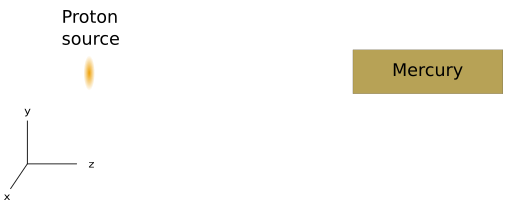
\includegraphics[scale=0.7]{../figs/mercury.png}
	\caption[VPI]{Planar view of Verification Problem I, 22 cm  x 44 cm x 186 cm}
	\label{fig:VPI}
\end{figure}
\begin{figure}[h!]
	\centering
	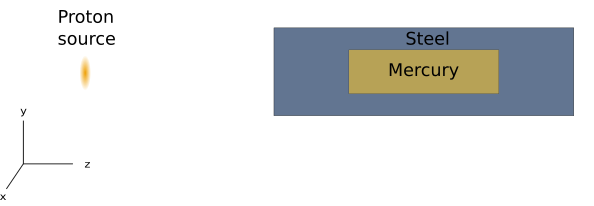
\includegraphics[scale=0.71]{../figs/mer_steel.png}
	\caption[VPI]{Planar view of Verification Problem II geometry, 44 cm x 88 cm x 372 cm}
	\label{fig:VPII}
\end{figure}

%
\subsection{Shut Down Dose Rate Workflow}
The patched \gls{dag}-\gls{mcnp}6 was used to
perform the neutron transport. The neutron flux and the radionuclide information
was collected on a cell, a 1x1x1 mesh, a 2x2x2 mesh, and a 4x4x4 mesh. All
meshes were uniformly distributed Cartesian meshes. In addition, each geometry
was divided into 8 and 64 equal parts. This was done to allow for direct
comparison to each the 2x2x2 and 4x4x4 meshes respectively.
Verification problem II required materials to be mixed when the geometry was
split into 8 equal parts.

The activation script was then used to search  and write the flux and radionuclide
information for each mesh voxel and geometric cell. A material file was also
written for each region. The script called CINDER90 and a CINDER90 run was
executed for each region.

The photon source script was then used to collect output from CINDER90 to
build a photon source file which can be used in lieu of a source card in the
photon transport. The geometry used for the photon transport was the original
version with a superimposed Cartesian mesh. The photon flux was tallied and
folded with flux-to-dose conversion factors to obtain the biological dose rate
in the mesh.
%
\subsection{Results}
\subsubsection{Verification Problem I}
Starting with the neutron transport step, the information collected on the
radionuclide tally was compared for the each of the meshes and the geometric
cell. For Verification problem I, the information collected in the mercury
volume was compared to the information collected in the 1x1x1 mesh as well
as to the sum of the results in each voxel of the 2x2x2 and 4x4x4 mesh. These
results can be seen in Figure \ref{fig:1prod_cell_1x_2x_4x}.
%
\begin{figure}[h!]
 \centering
 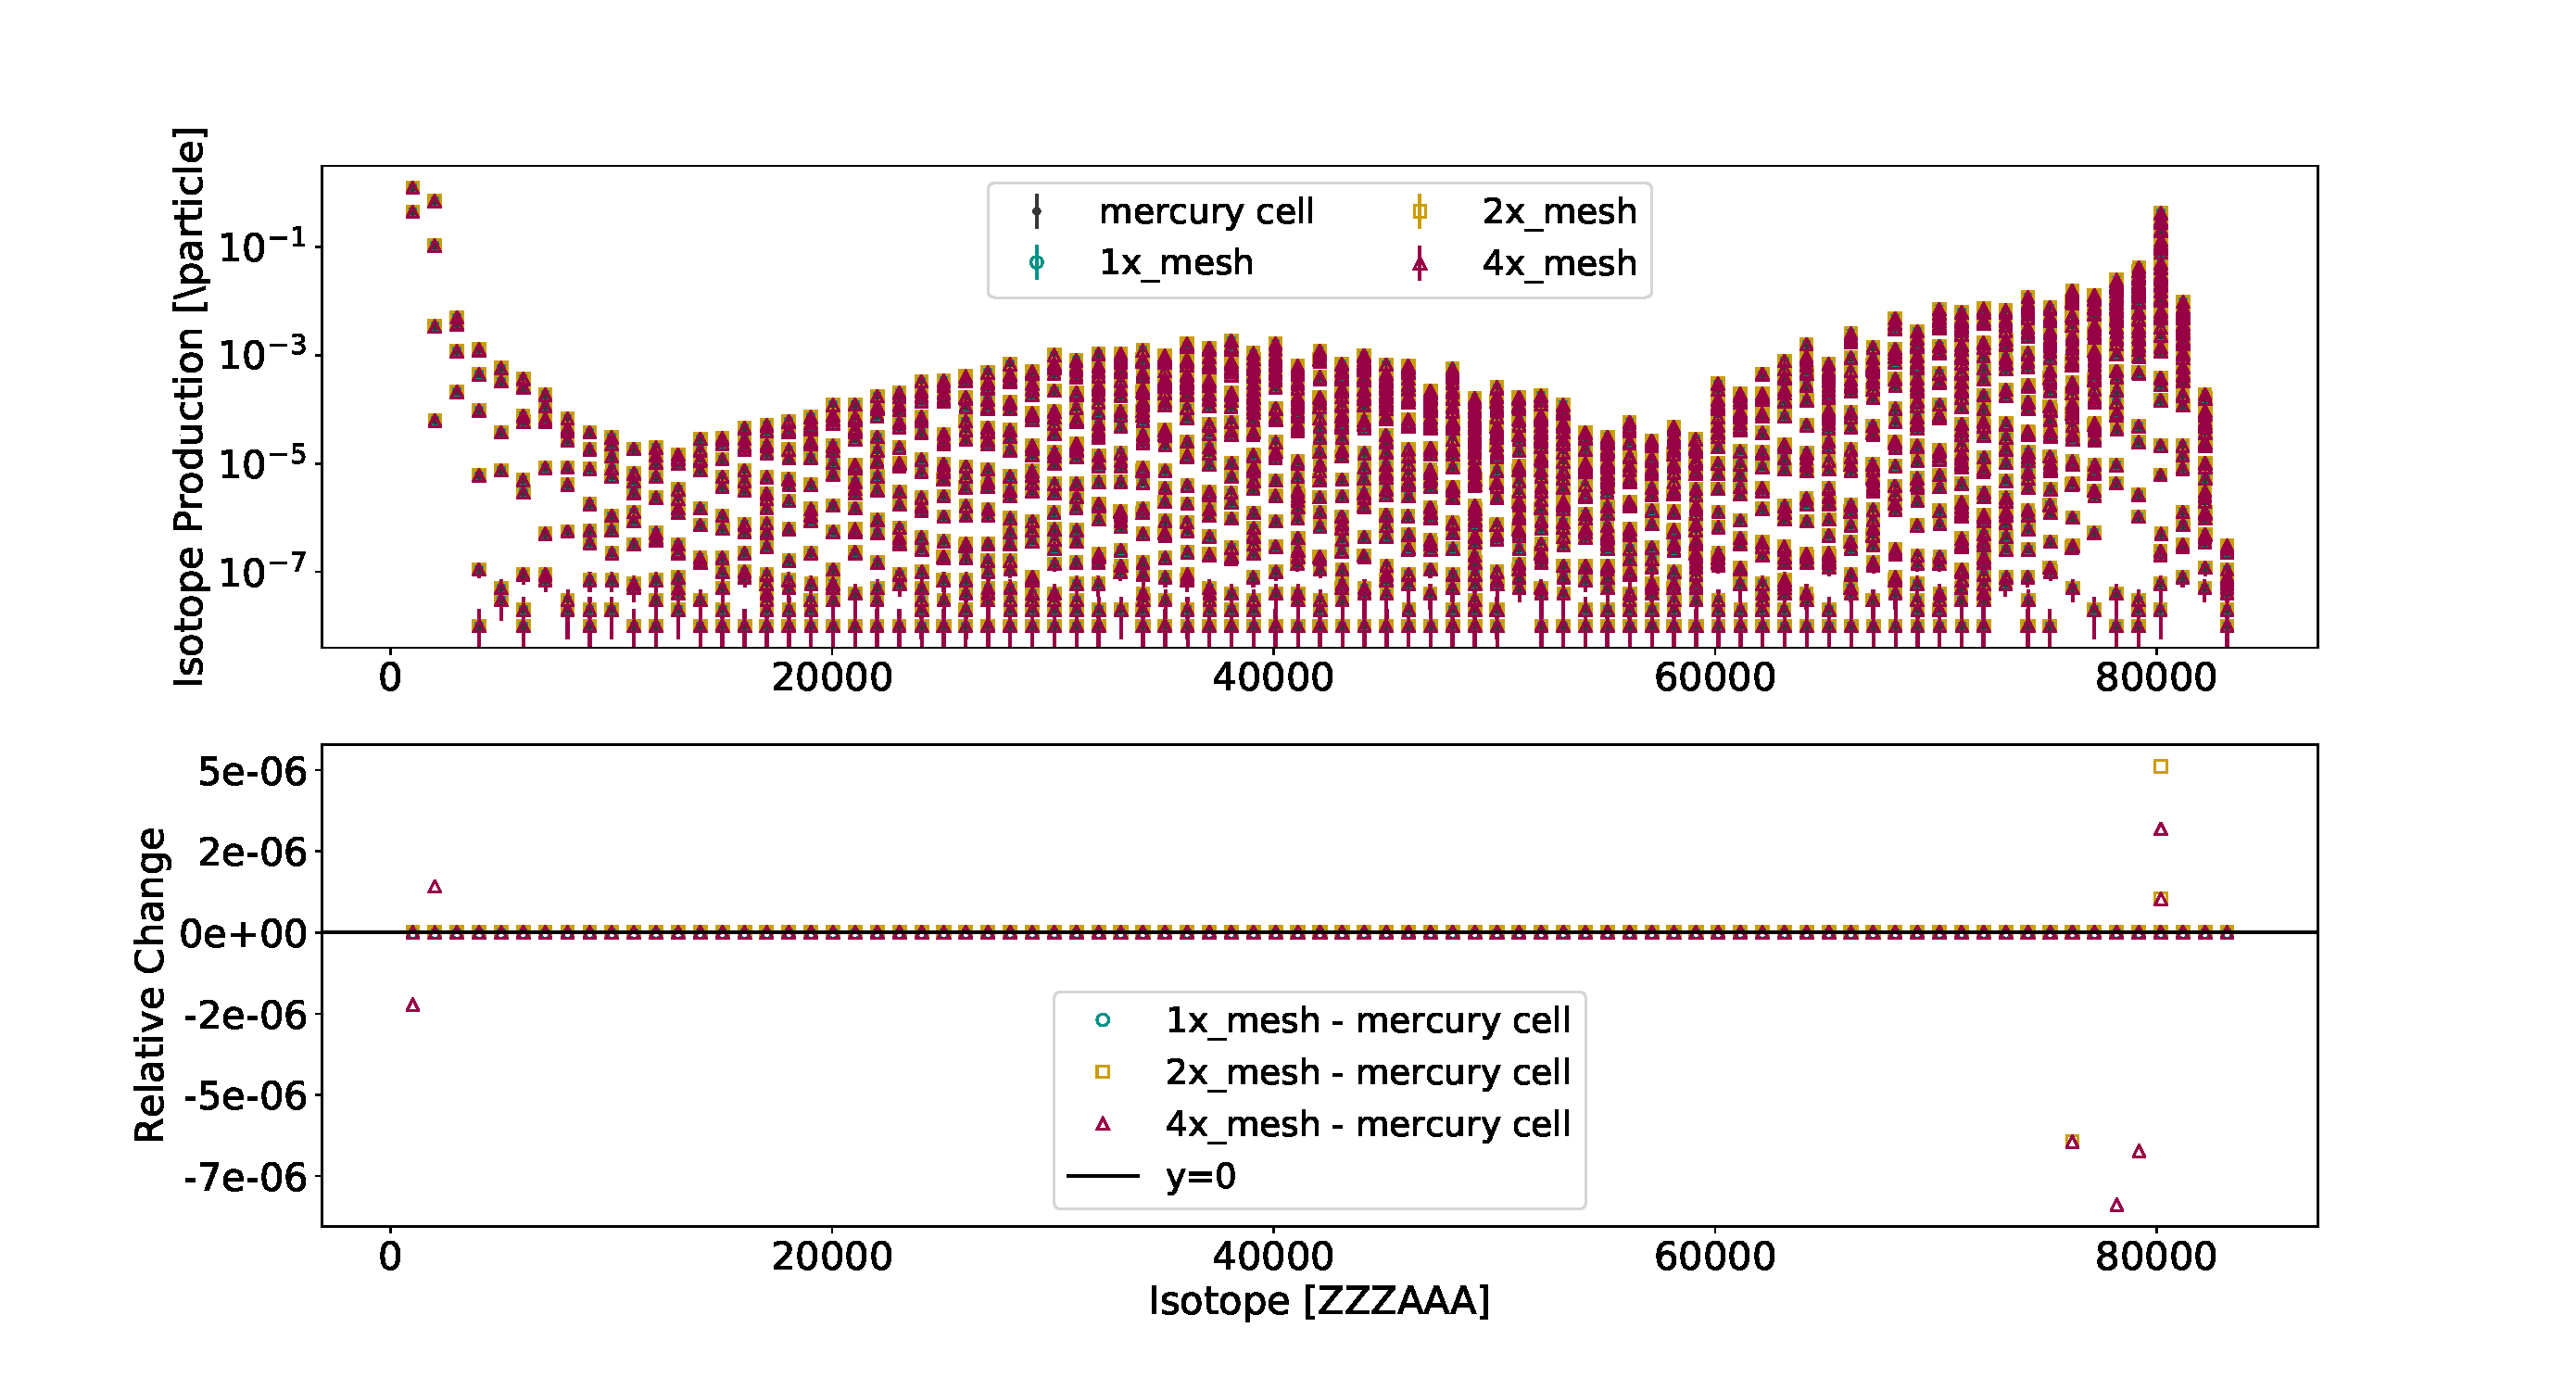
\includegraphics[scale=0.42,trim={2cm 1cm 3cm 2cm},clip]{../figs/toy_p1/prod_VPI_1x_2x_4x.pdf}
 \caption{Radionuclide production comparison for mercury cell and different meshes}
 \label{fig:1prod_cell_1x_2x_4x}
\end{figure}
%
\\
Figure \ref{fig:1prod_cell_2x} compares the results collected in the geometric
cell, the summed up results of the 2x2x2 mesh and the 2x2x2 divided geometry.
%
\begin{figure}[h!]
 \centering
 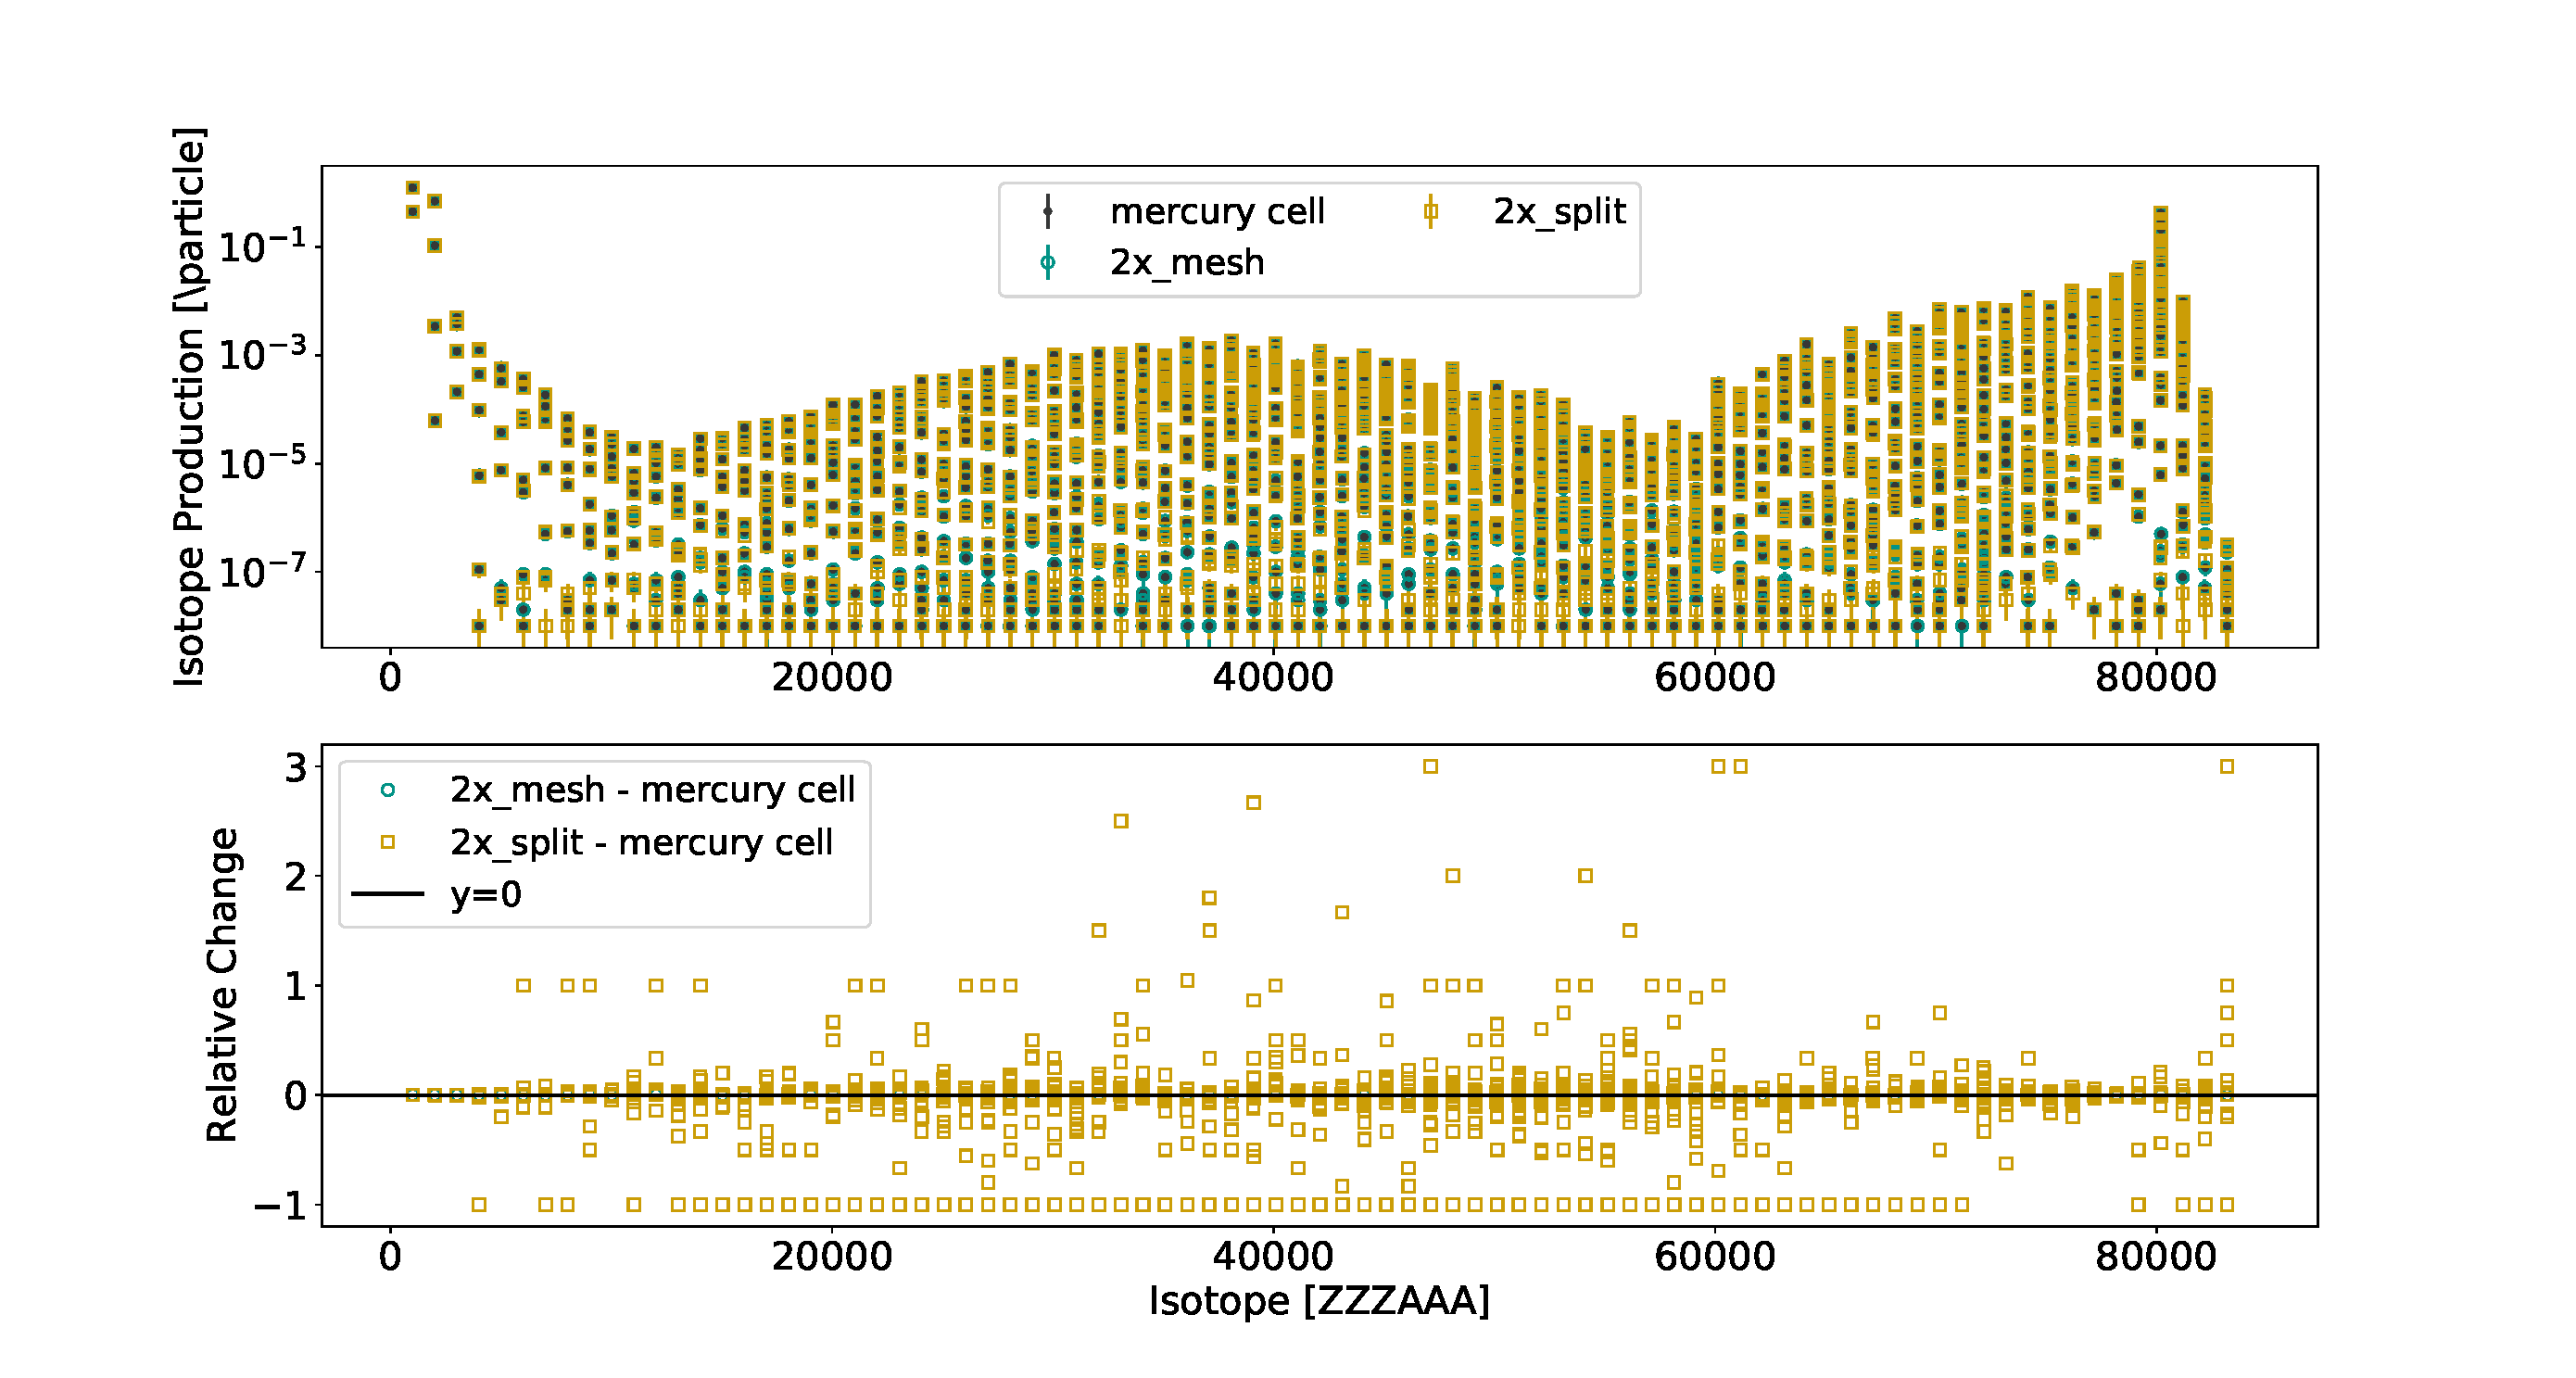
\includegraphics[scale=0.42,trim={3cm 1cm 3cm 3cm},clip]{../figs/toy_p1/prod_VPI_2x.pdf}
 \caption{Radionuclide production comparison between mercury cell, 2x2x2 mesh and geometry split}
 \label{fig:1prod_cell_2x}
\end{figure}
%
\\
A similar comparison was made for the 4x4x4 mesh and the 4x4x4 divided geometry
which can be seen in Figure \ref{fig:1prod_cell_4x}
%
\begin{figure}[h!]
 \centering
 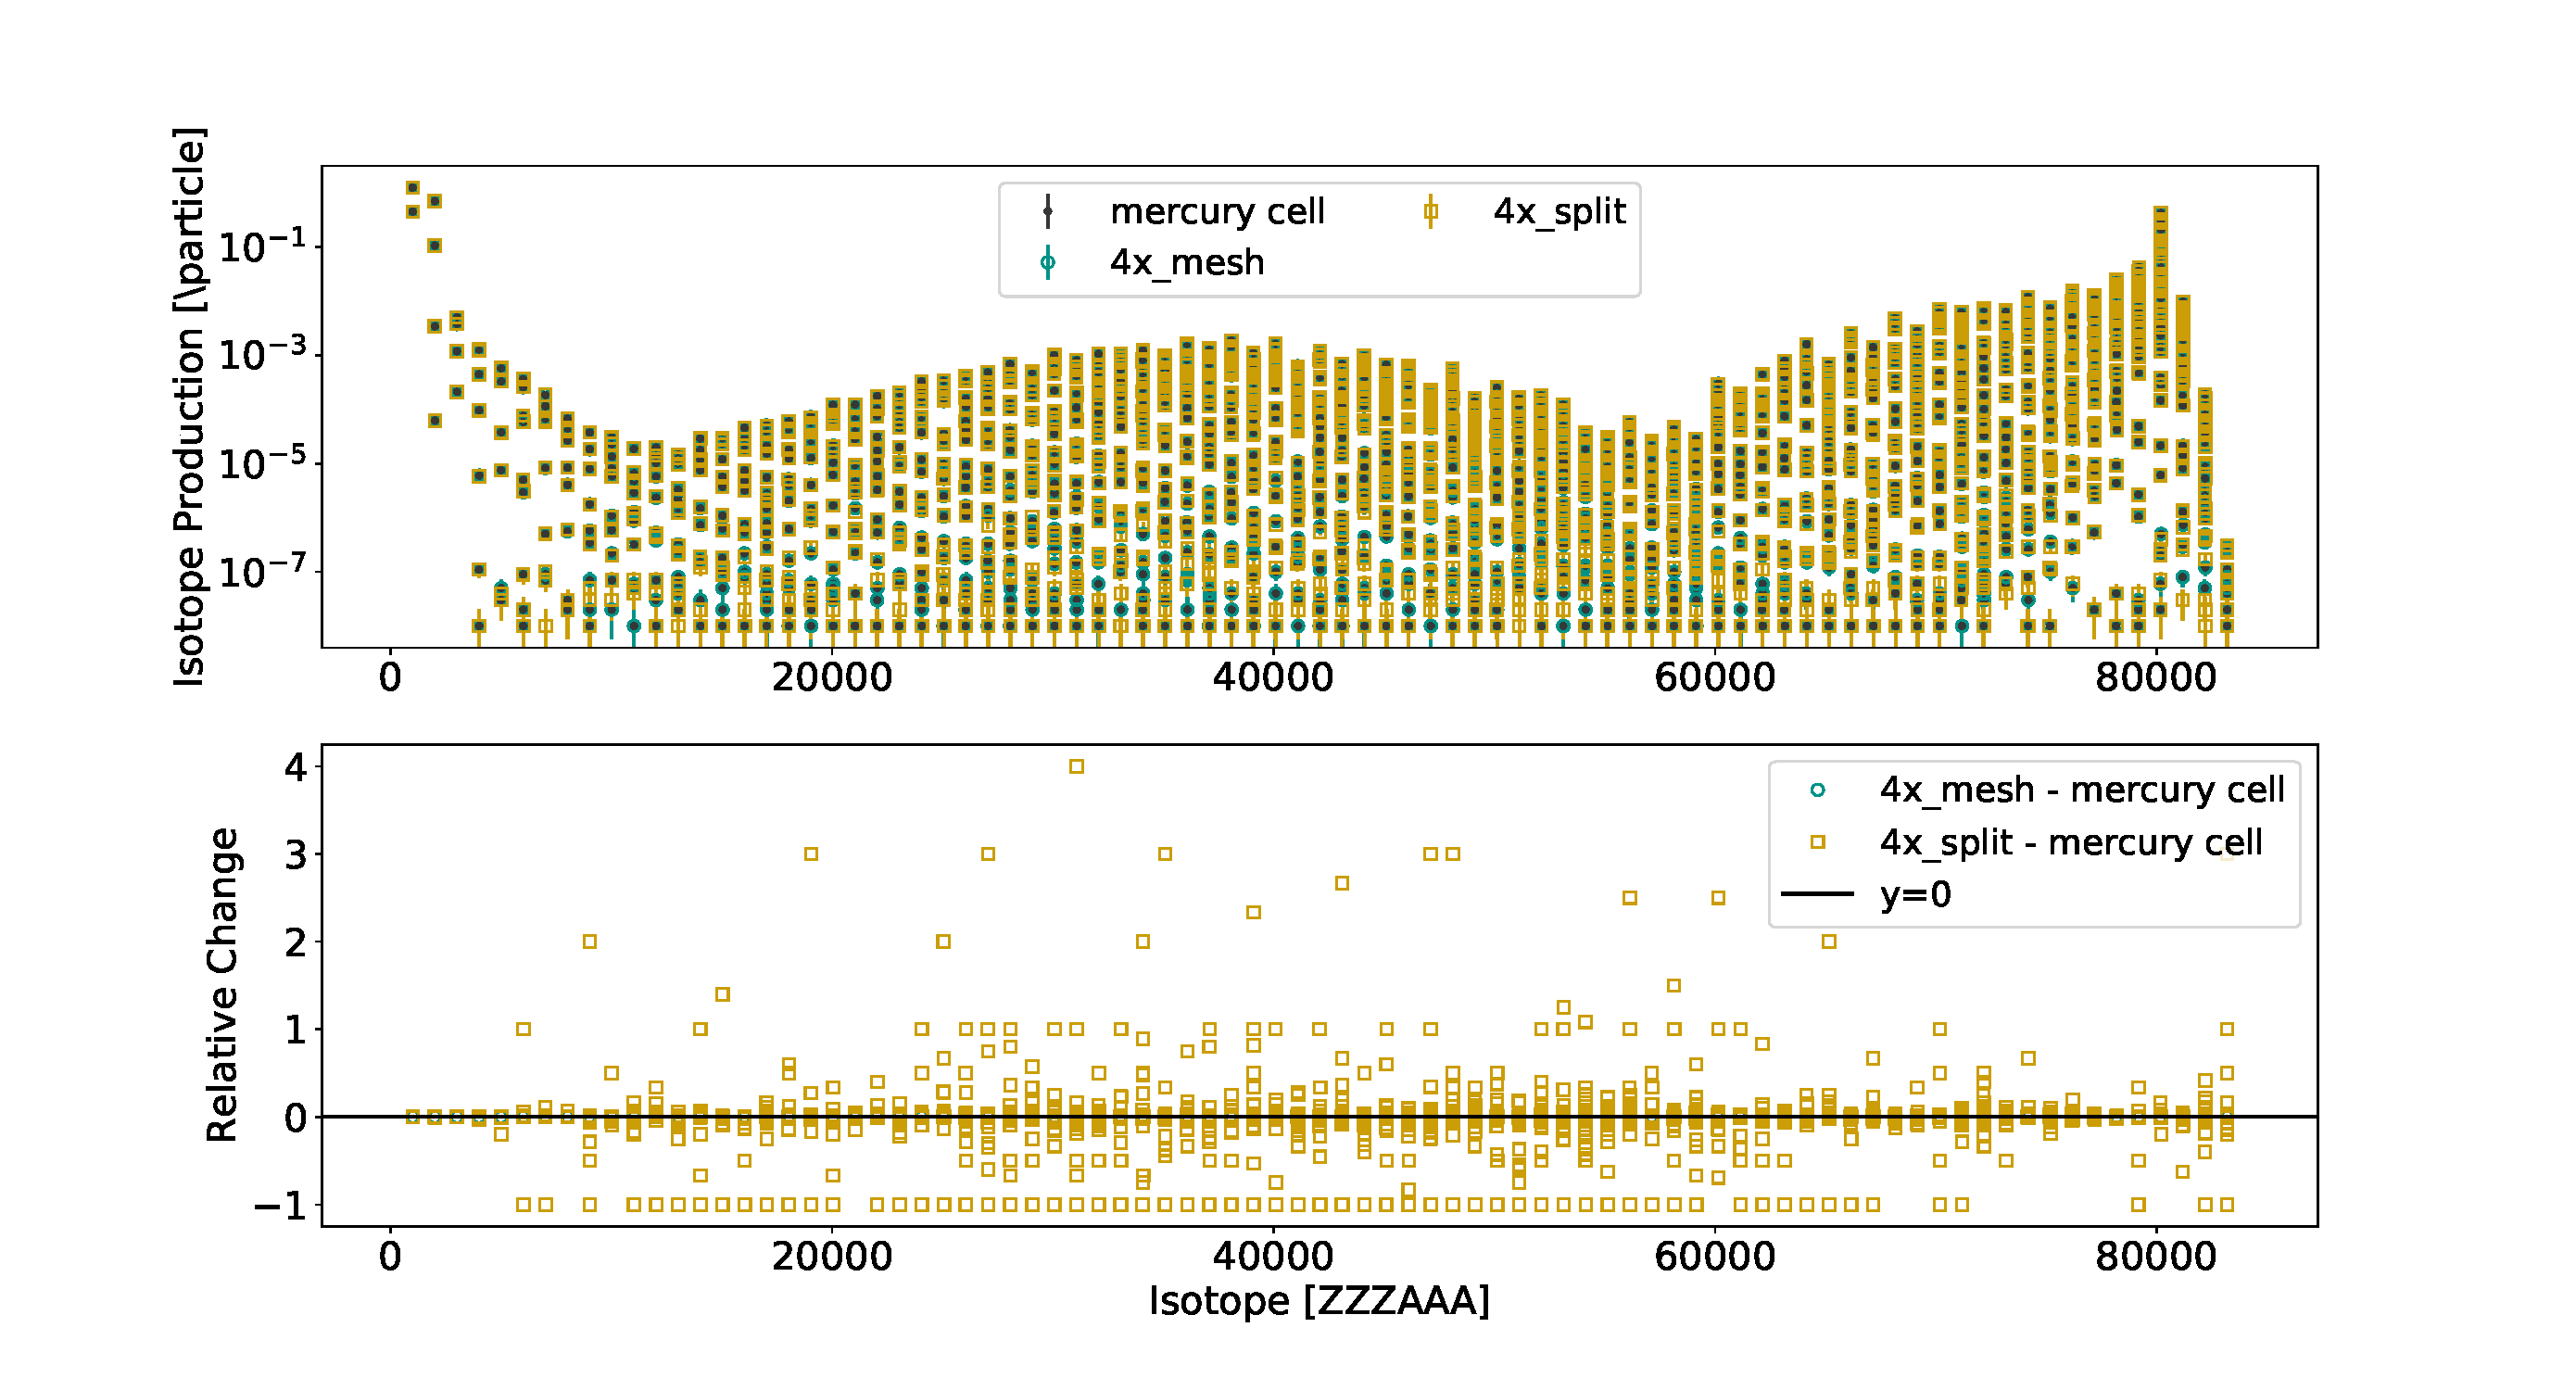
\includegraphics[scale=0.42,trim={3cm 1cm 3cm 3cm},clip]{../figs/toy_p1/prod_VPI_4x.pdf}
 \caption{Radionuclide production comparison between mercury cell, 4x4x4 mesh and geometry split}
 \label{fig:1prod_cell_4x}
\end{figure}
%
\\
Figure \ref{fig:1prod_cell_1x_2x_4x} shows some differences between the
results for the mesh and the results collected in the mercury cell. Figure
\ref{fig:1prod_cell_2x} and \ref{fig:1prod_cell_4x} show bigger difference when
comparing the mercury cell to the results of the divided geometry.\\
Figure \ref{fig:1prod_cell_2x_rc} and \ref{fig:1prod_cell_4x_rc} show the
relative change between the results collected in the geometric volume and the
one collected for the split geometry versus the results collected for the cell.
In both graphs, one can see that the relative change is large when the isotope
production per particle is low. This is important to note since these low
production isotopes might be less important to the photon source.
%
\begin{figure}[h!]
 \centering
 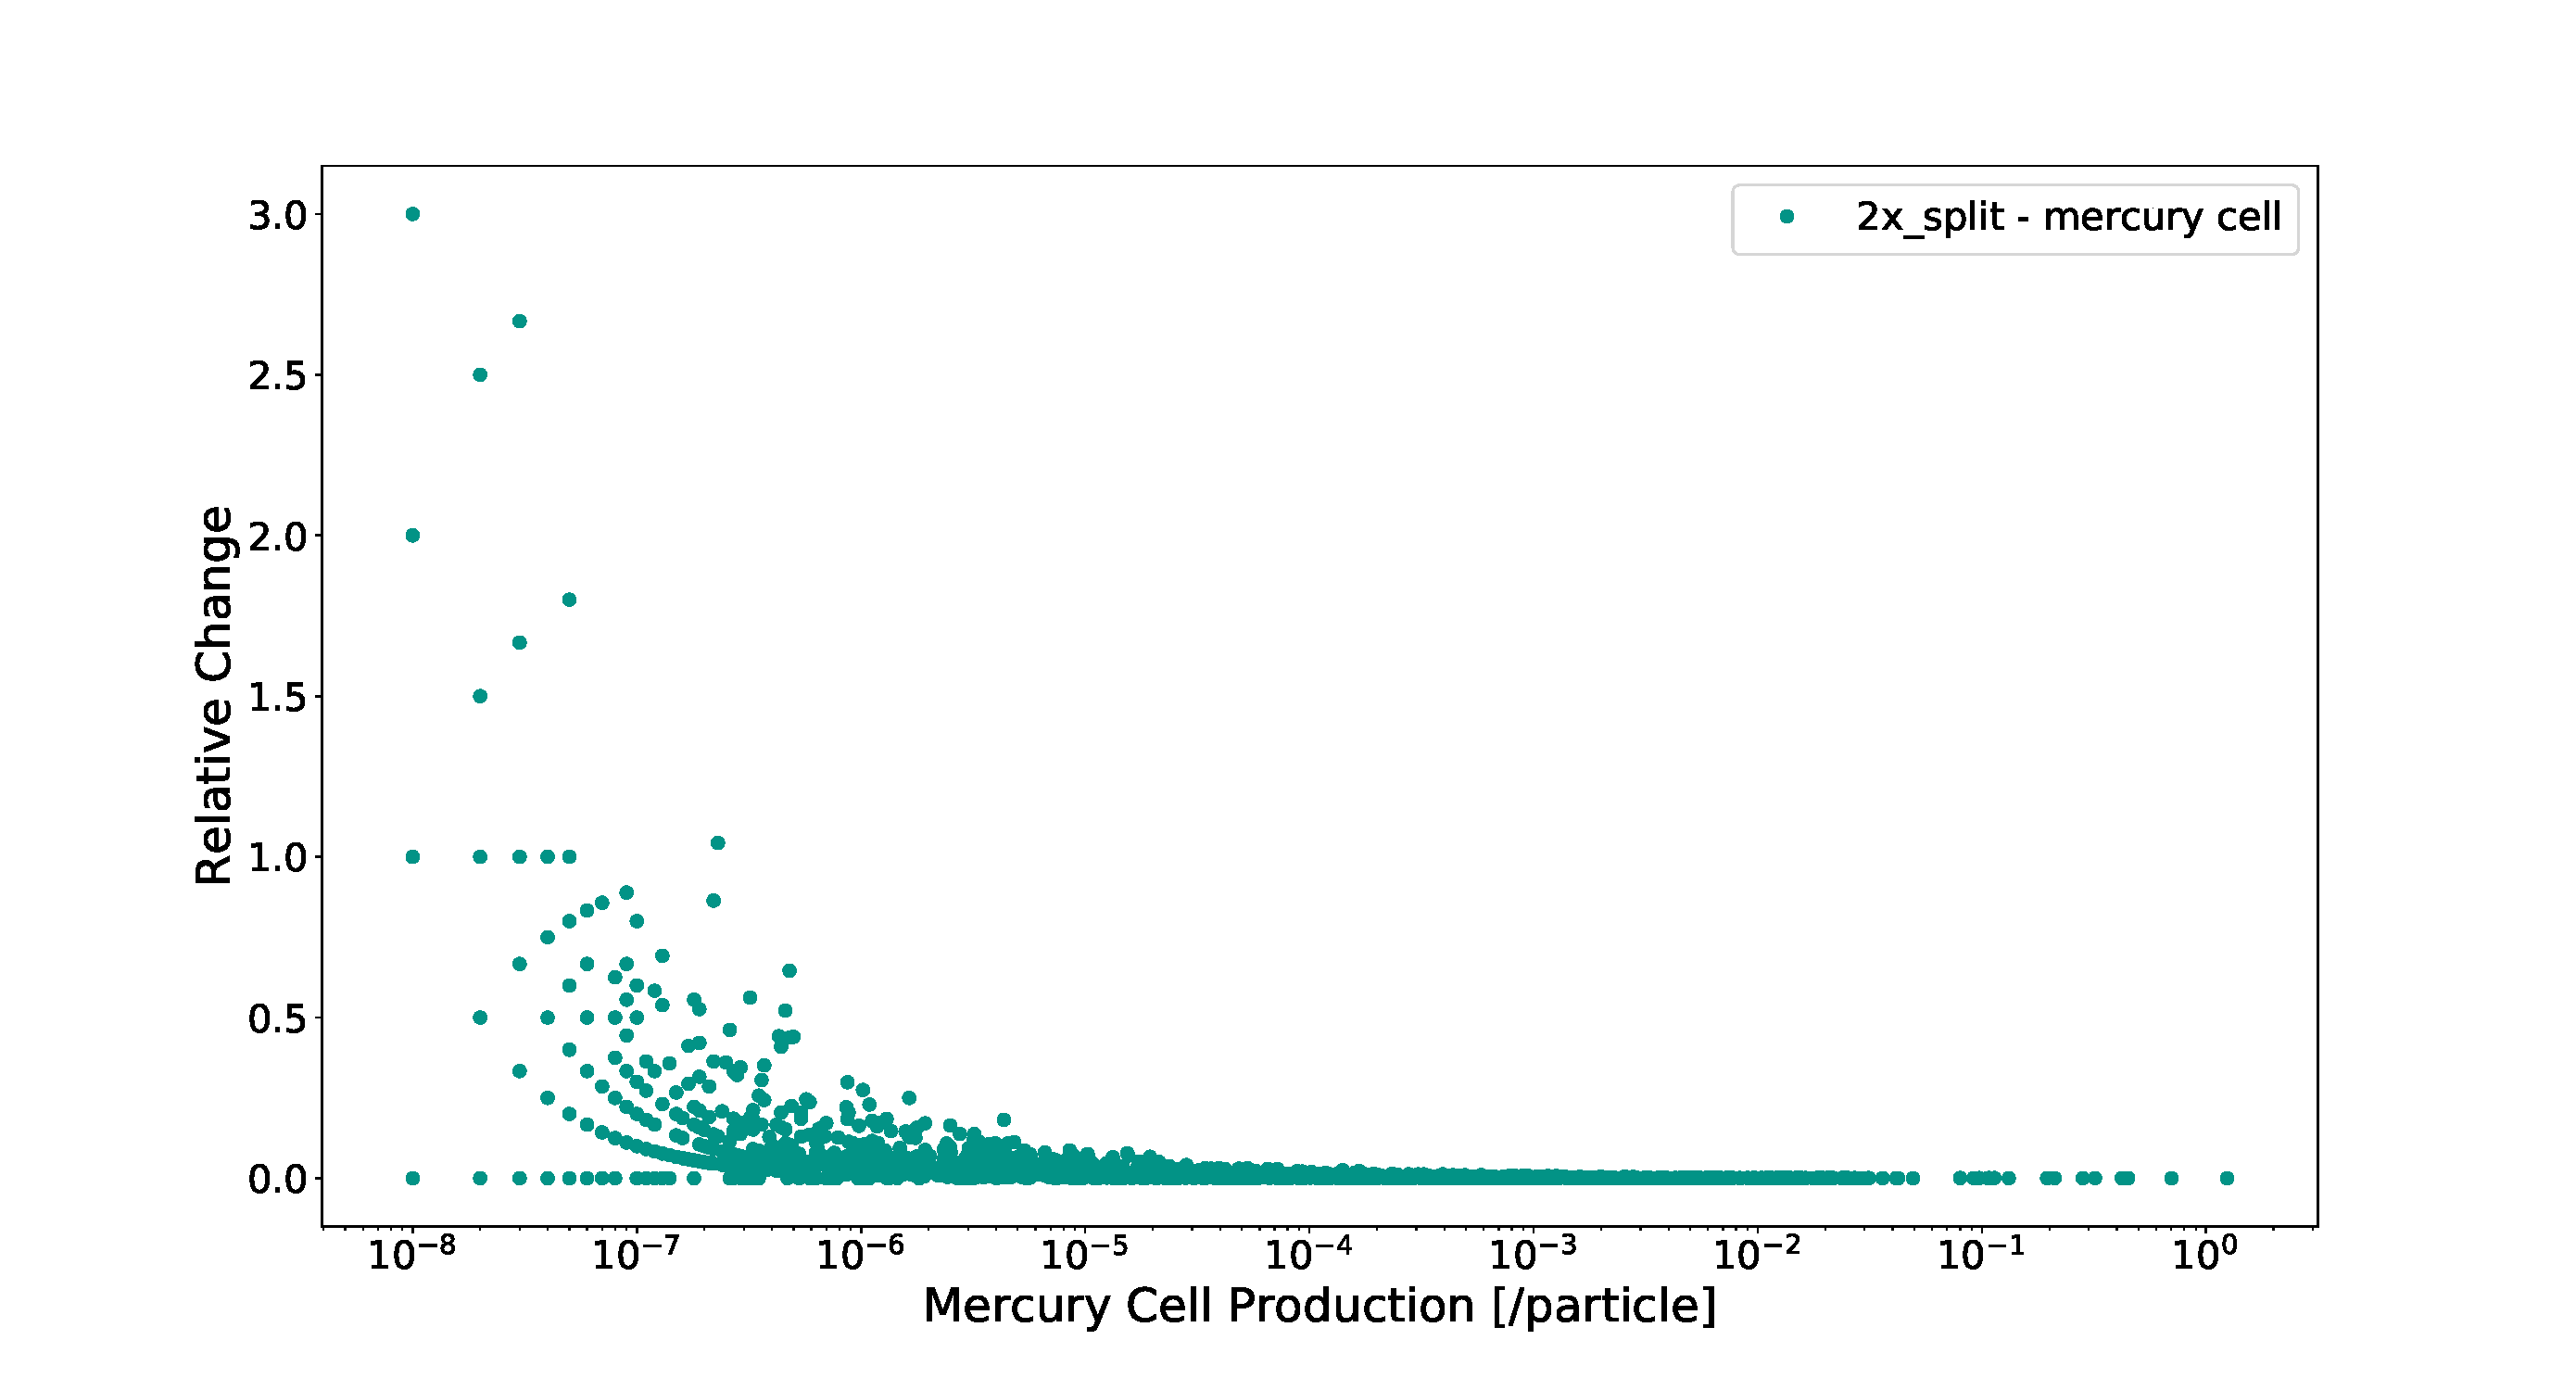
\includegraphics[scale=0.42,trim={3cm 0.5cm 3cm 3cm},clip]{../figs/toy_p1/prod_VPI_rc_2x_split.pdf}
 \caption{Relative change between mercury cell and 2x2x2 geometry split vs. the isotope production of the mercury cell}
 \label{fig:1prod_cell_2x_rc}
\end{figure}
\begin{figure}[h!]
 \centering
 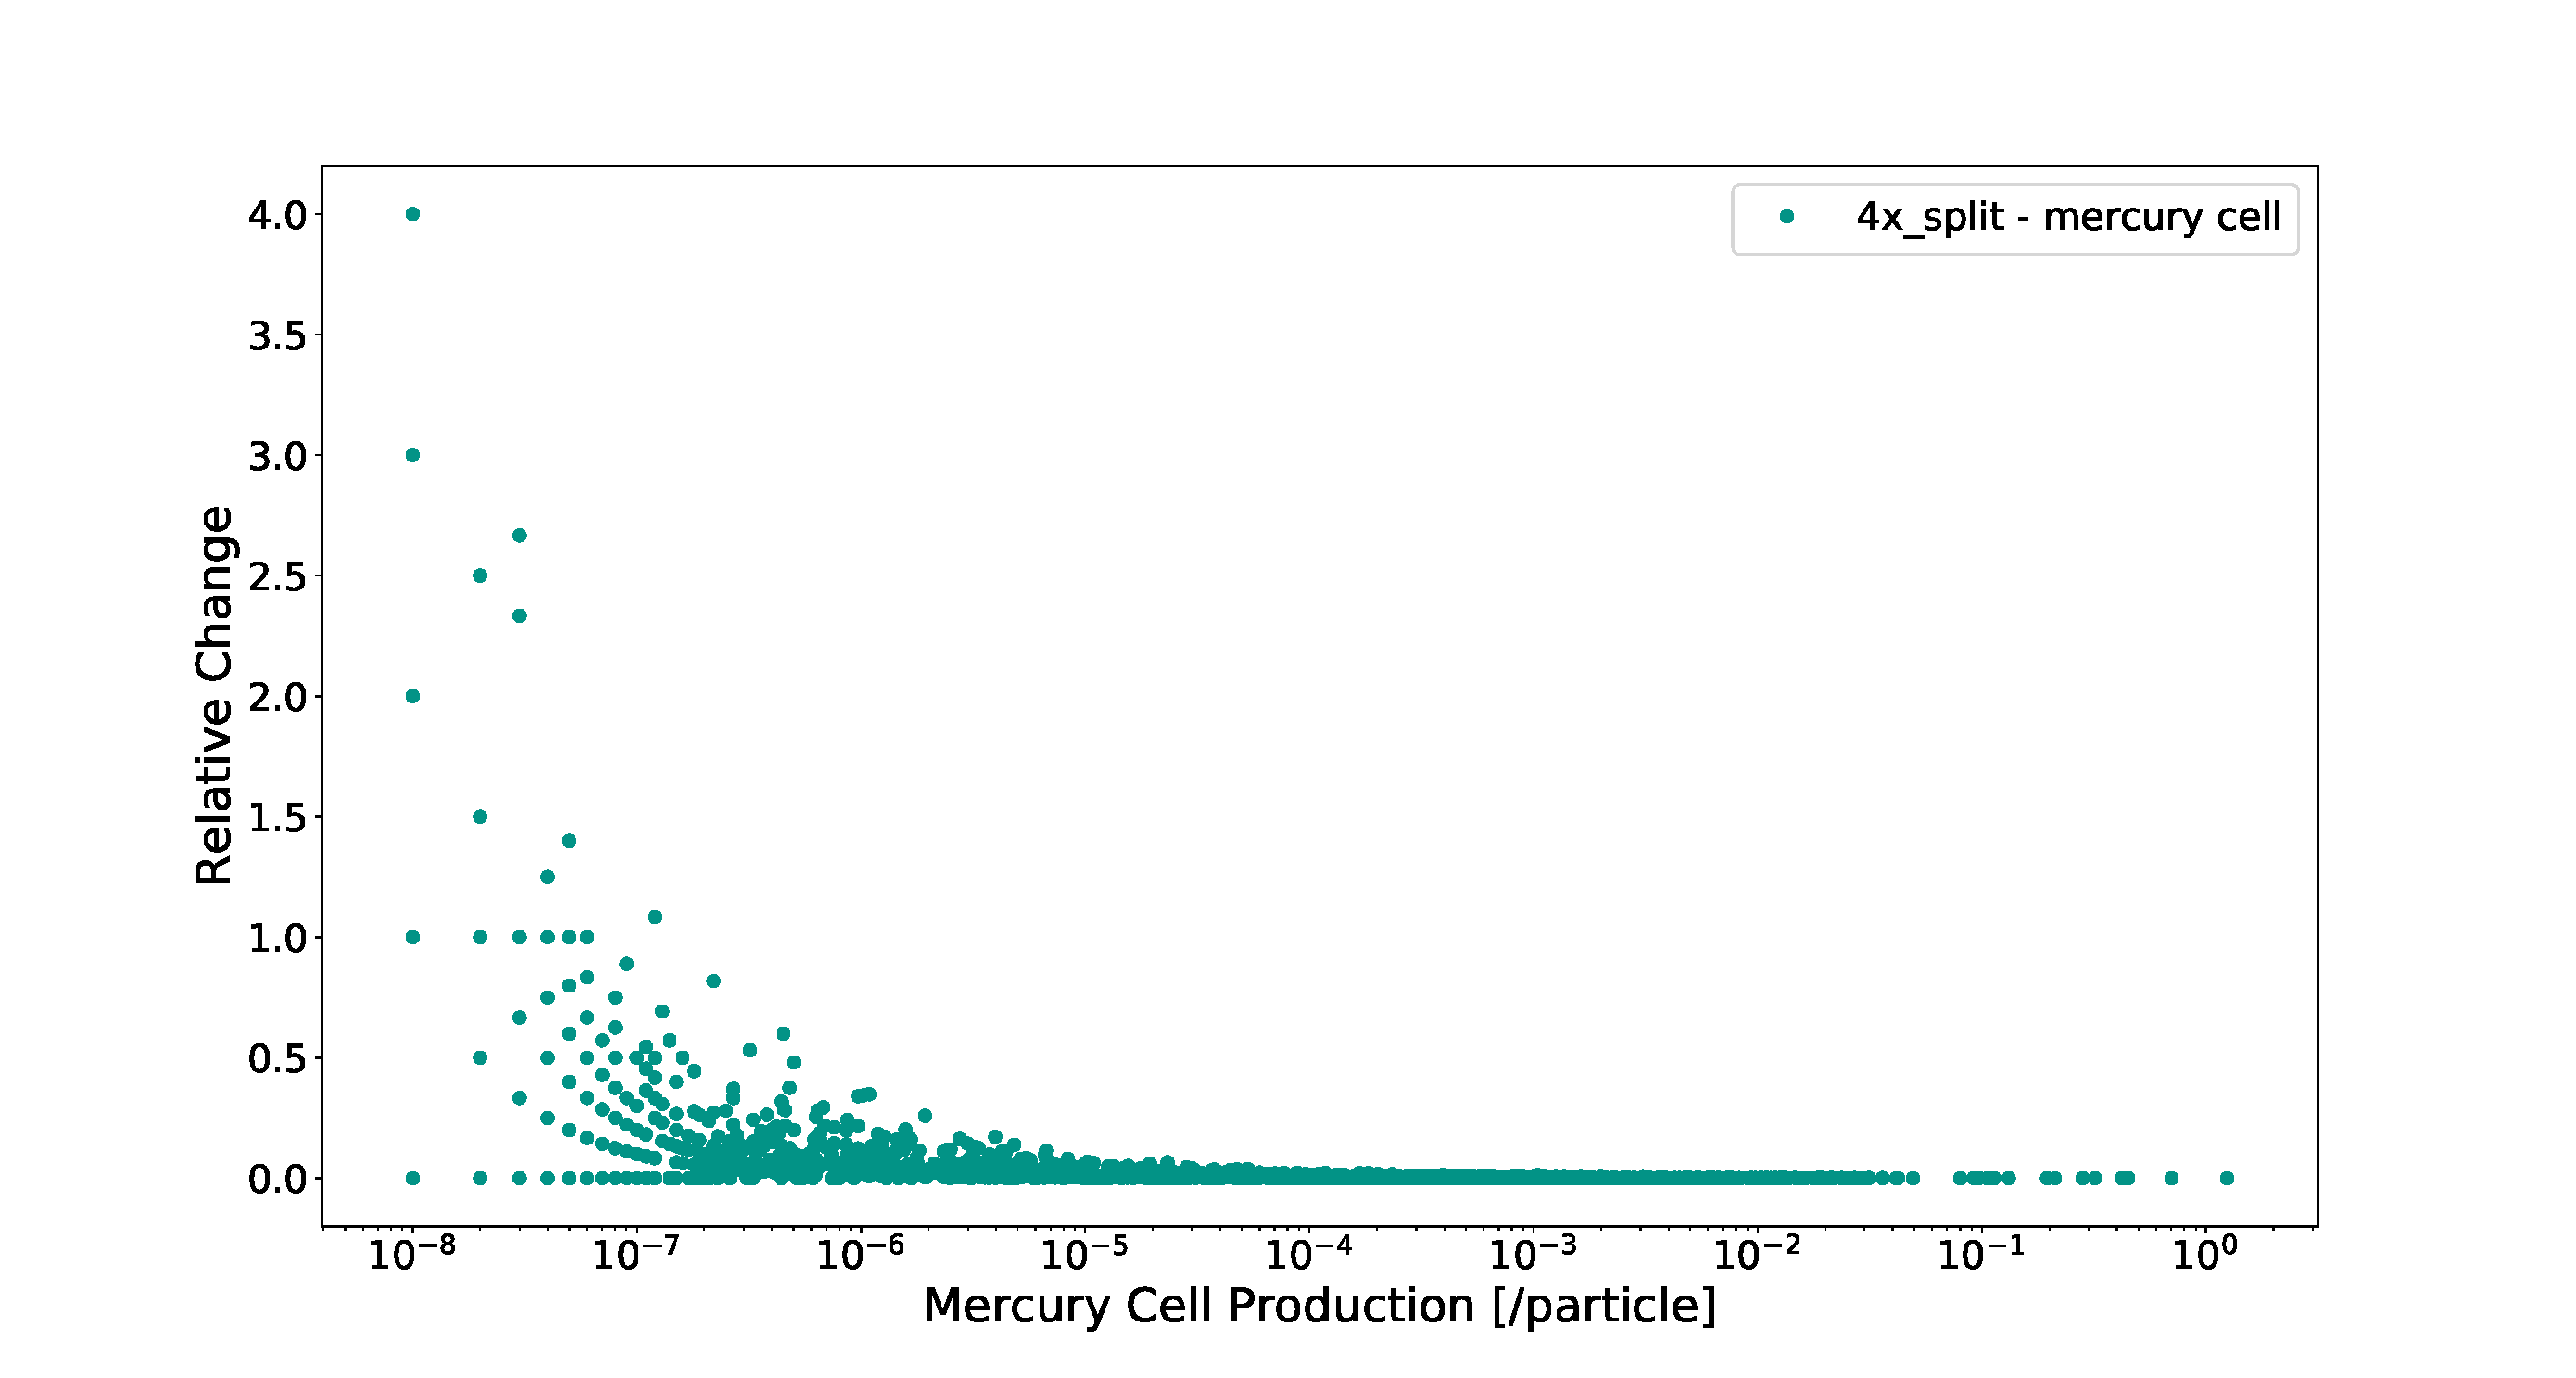
\includegraphics[scale=0.42,trim={3cm 0.5cm 3cm 3cm},clip]{../figs/toy_p1/prod_VPI_rc_4x_split.pdf}
 \caption{Relative change between mercury cell and 4x4x4 geometry split vs. the isotope production of the mercury cell}
 \label{fig:1prod_cell_4x_rc}
\end{figure}
%
\\
For the activation step of the workflow, an activation calculation was run for
each problem. The results obtained with information collected in the mercury
cell were compared to results collected in the different meshes and can be seen
in Figure \ref{fig:1spec_cell_1x_2x_4x}. Results were average between all voxels
in a mesh to be able to compare directly to the cell results.
%
\begin{figure}[h!]
 \centering
 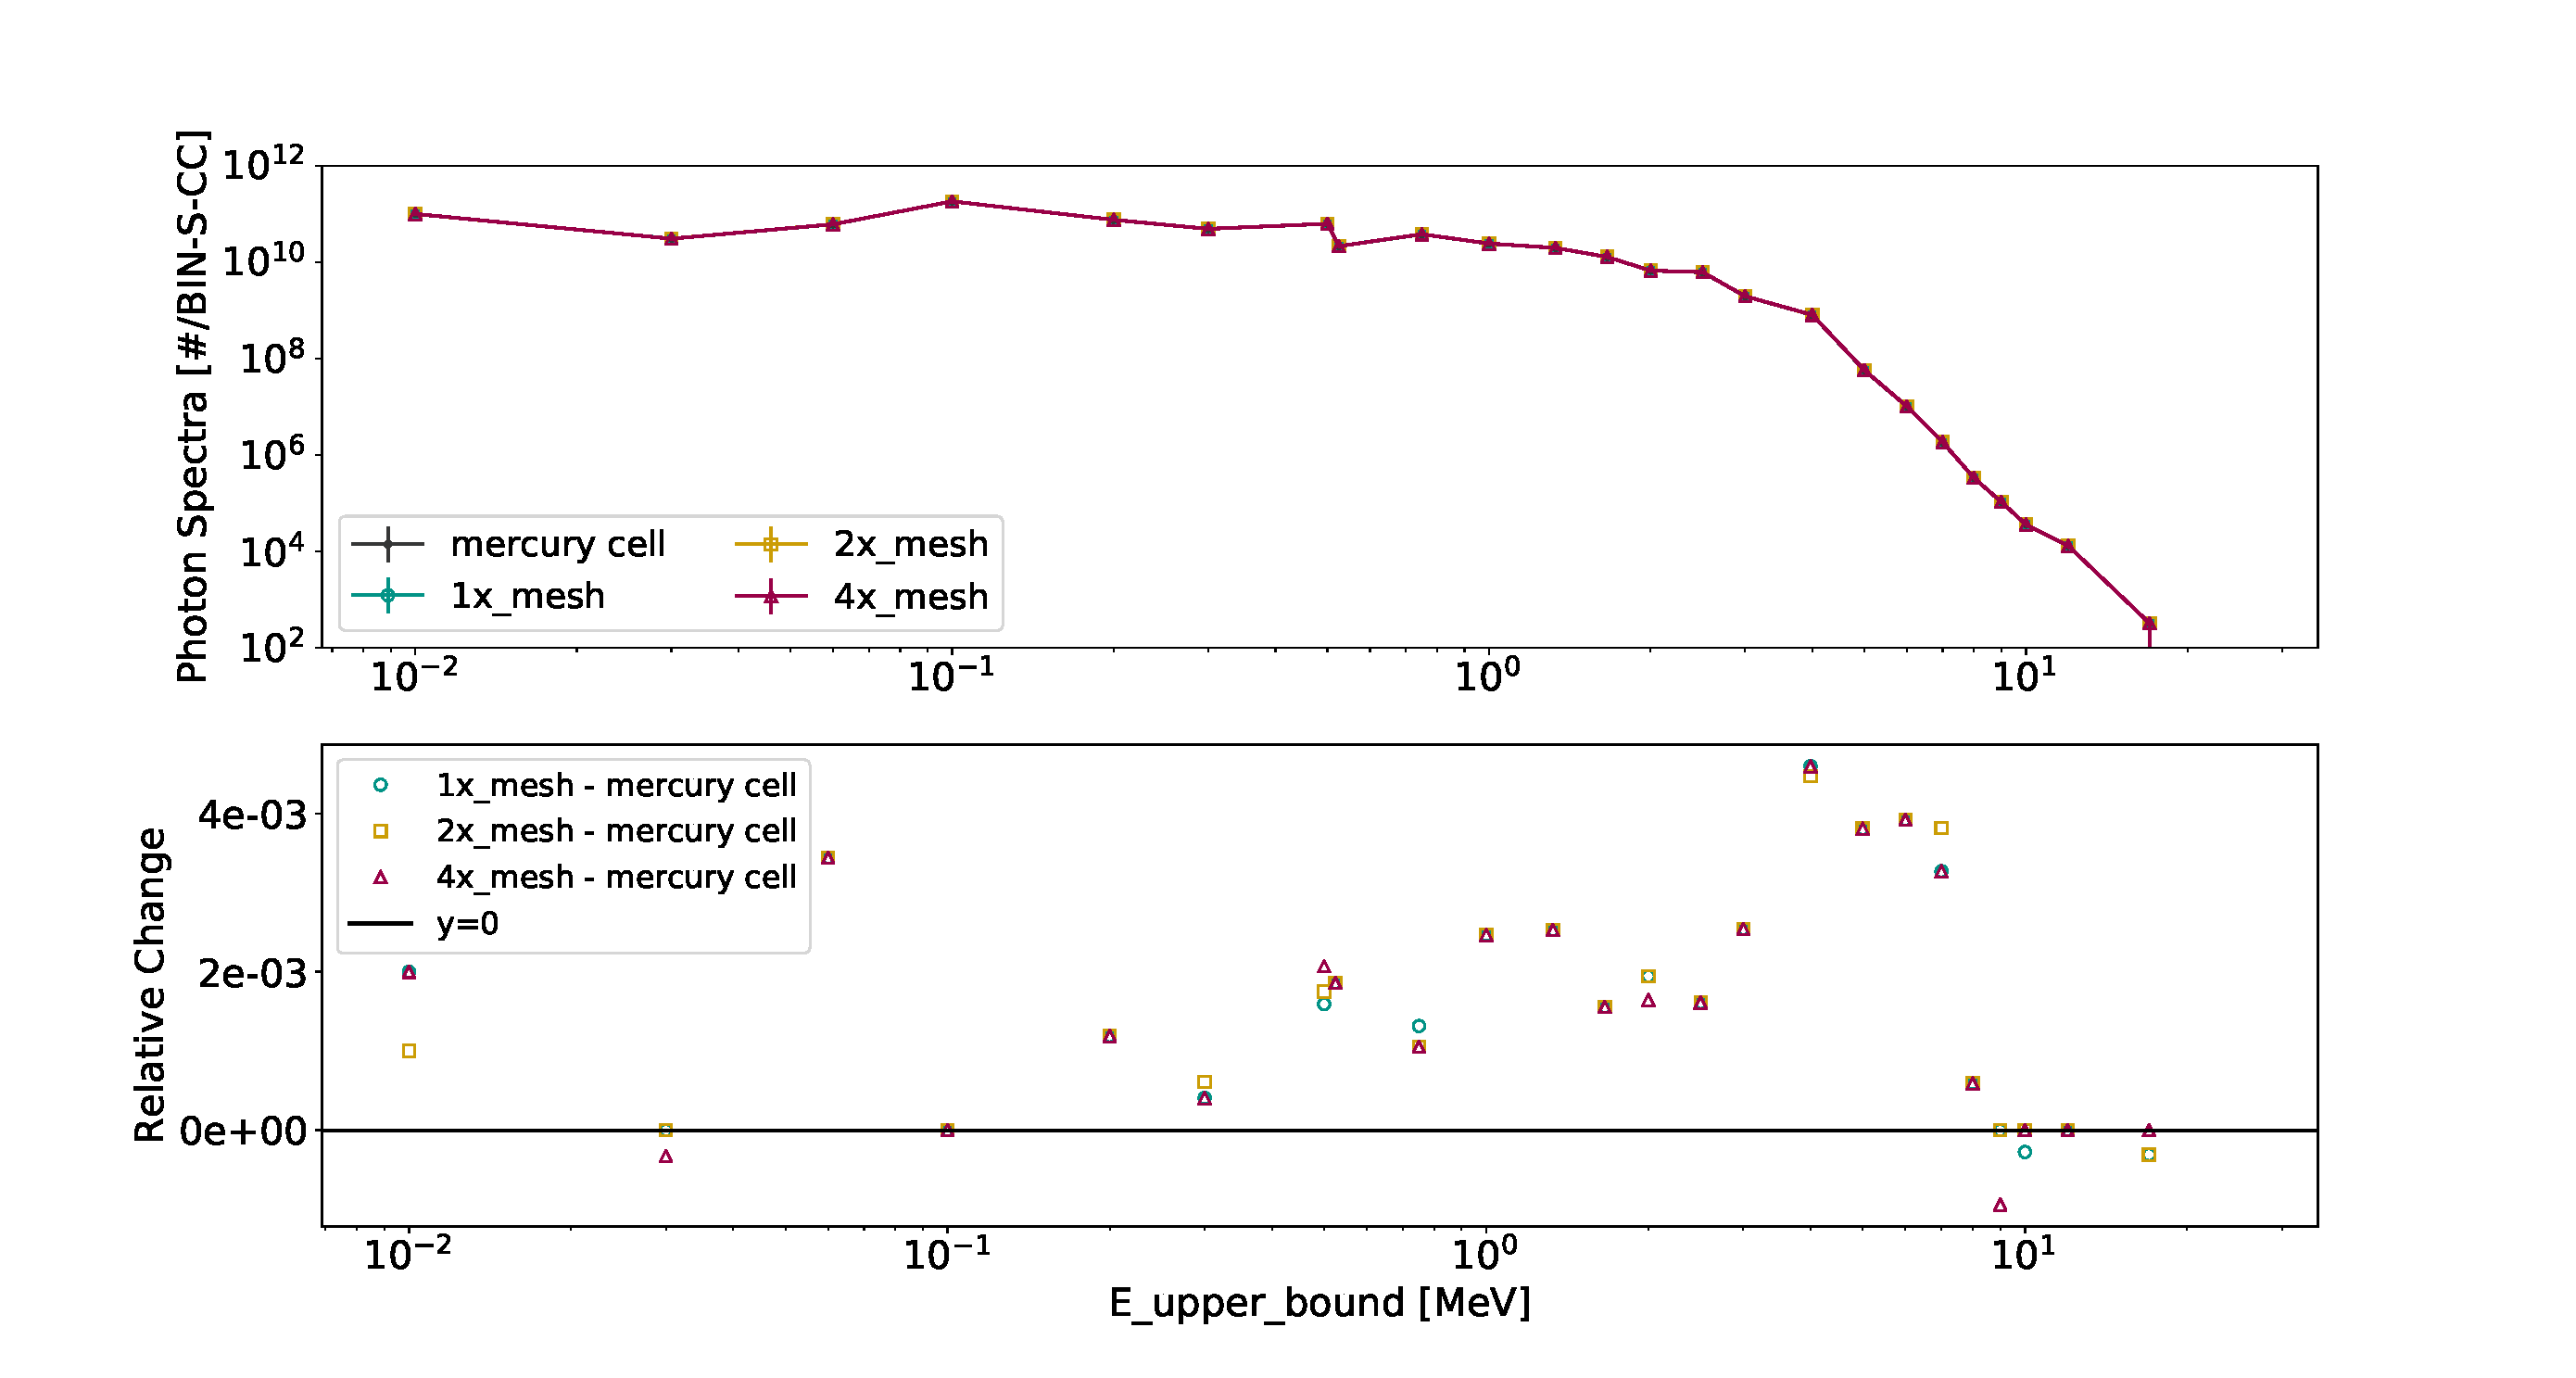
\includegraphics[scale=0.42,trim={2cm 0.5cm 3cm 2cm},clip]{../figs/toy_p1/spec_VPI_1x_2x_4x.pdf}
 \caption{Photon Spectrum in mercury cell and different meshes}
 \label{fig:1spec_cell_1x_2x_4x}
\end{figure}
%
A comparison between the results in the mesh and the split geometry can be seen
in Figure \ref{fig:1spec_cell_2x} and \ref{fig:1spec_cell_4x}.
%
\begin{figure}[h!]
 \centering
 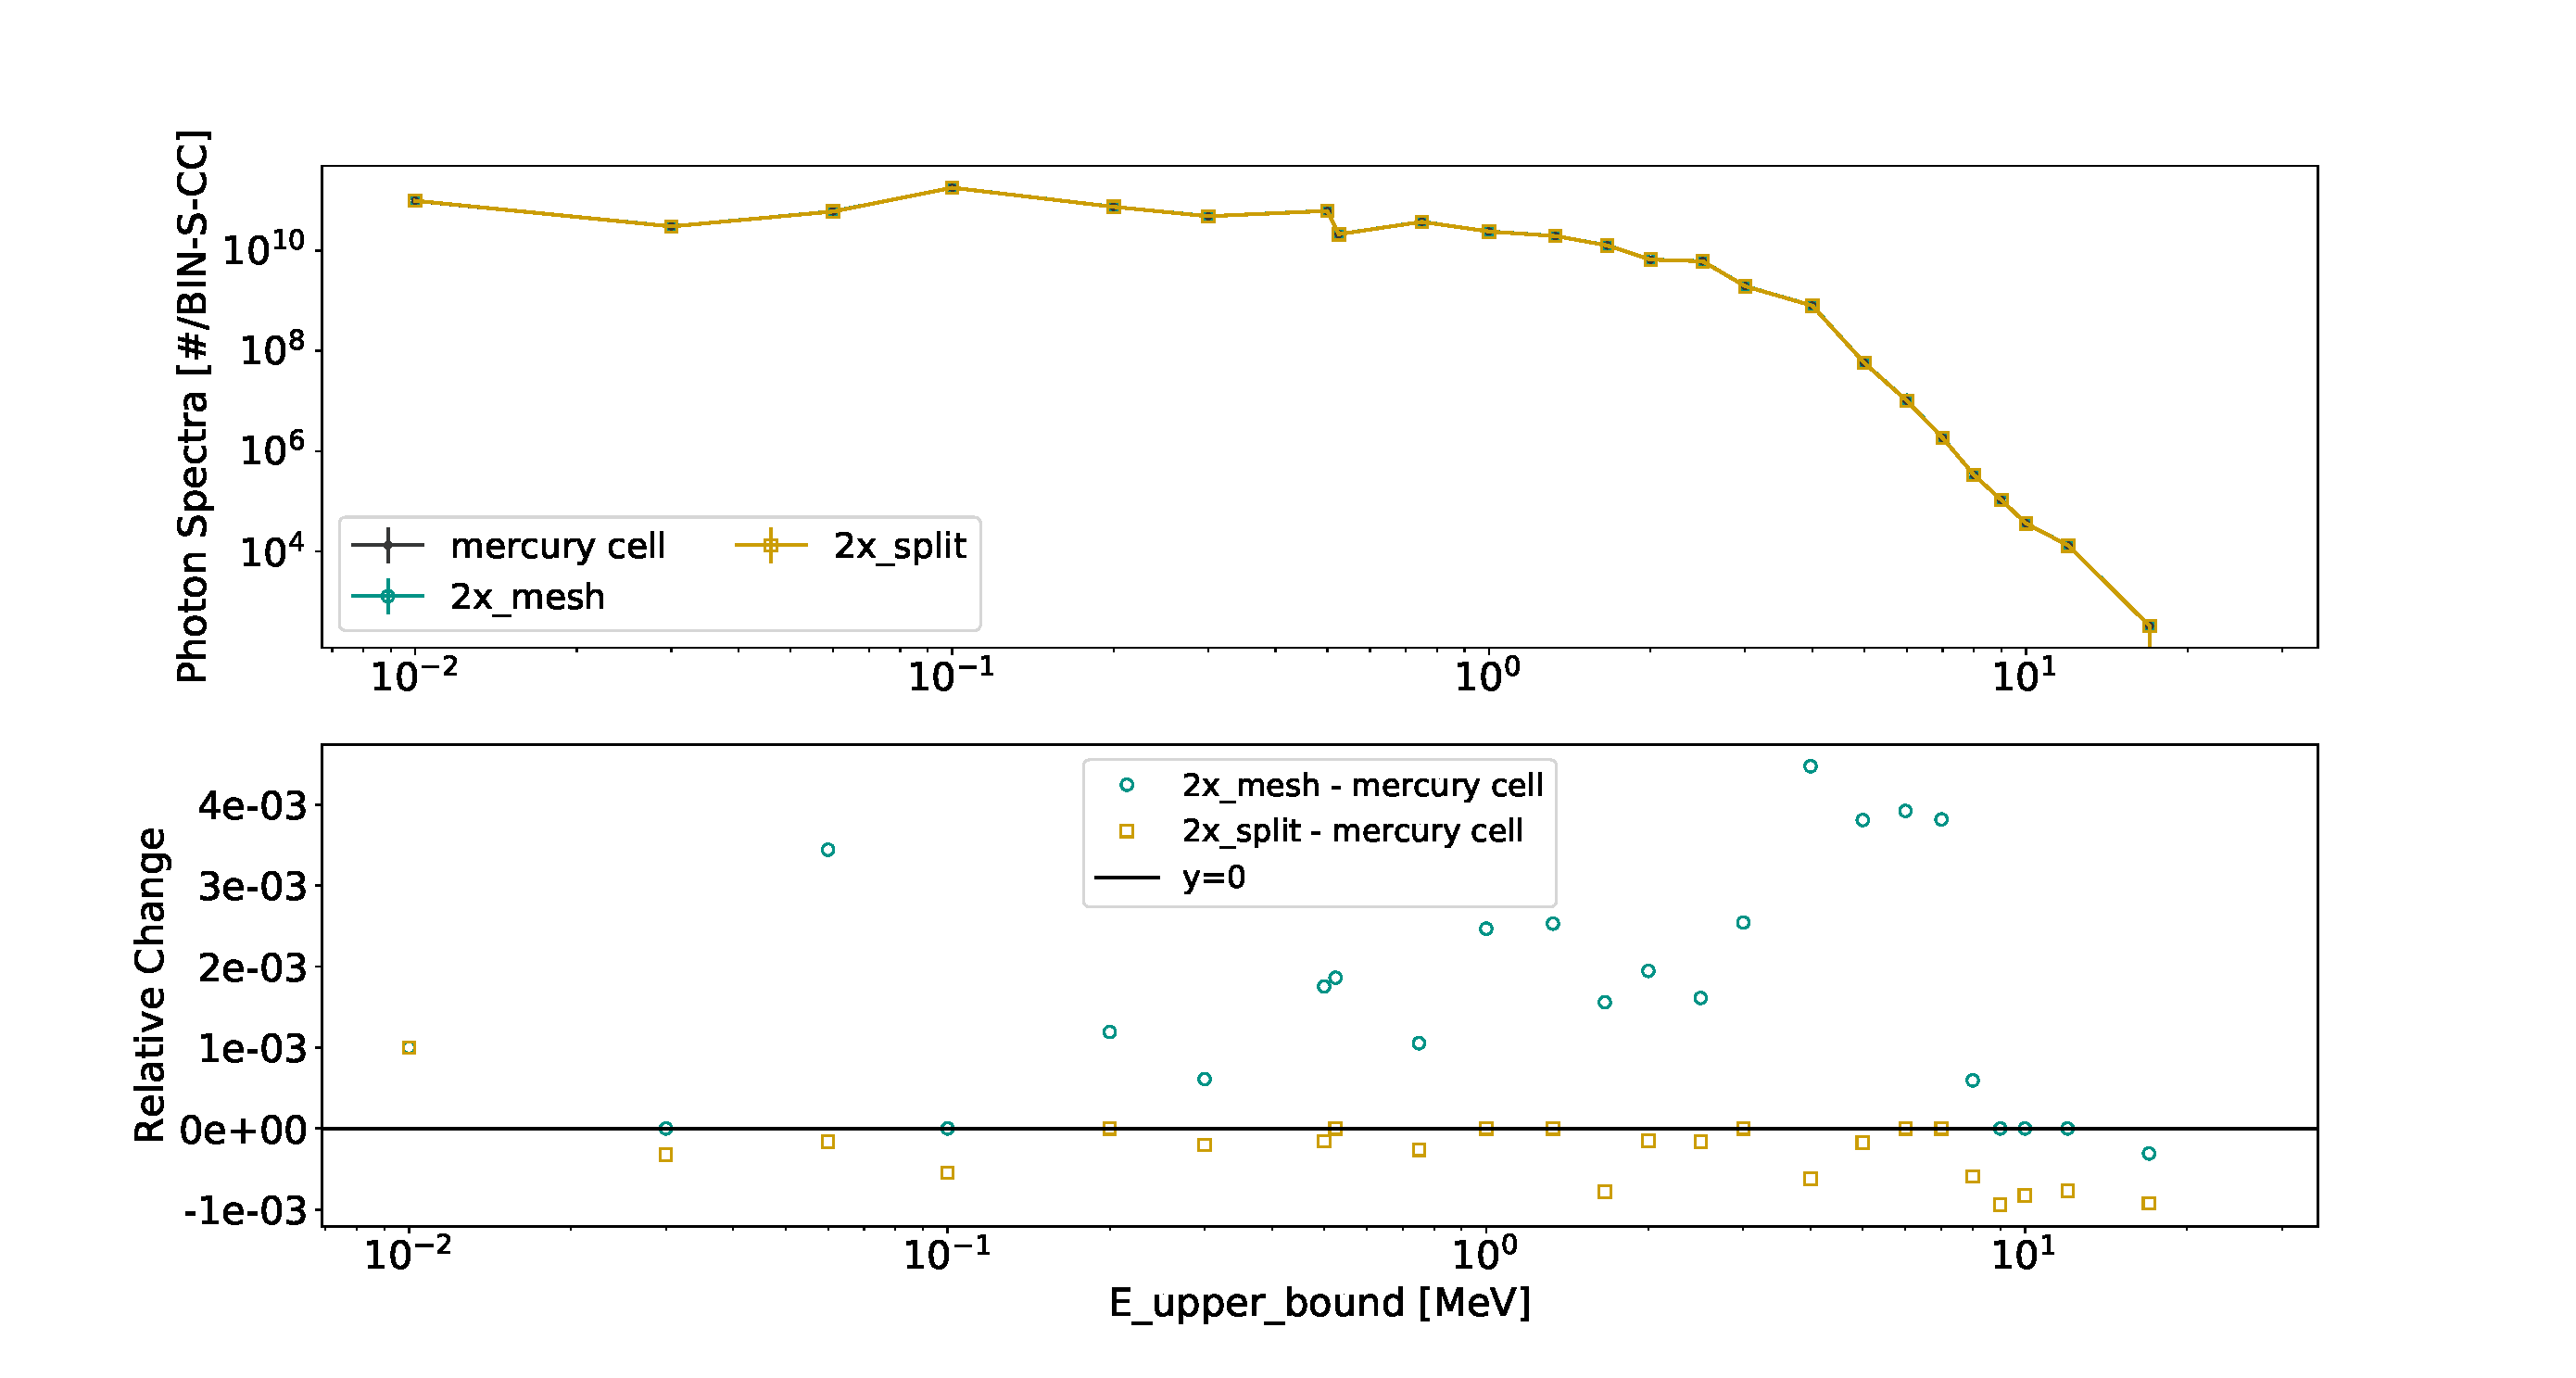
\includegraphics[scale=0.42,trim={3cm 1cm 3cm 3cm},clip]{../figs/toy_p1/spec_VPI_2x.pdf}
 \caption{Photon Spectrum in mercury cell, 2x2x2 mesh, and geometry split}
 \label{fig:1spec_cell_2x}
\end{figure}
\begin{figure}[h!]
 \centering
 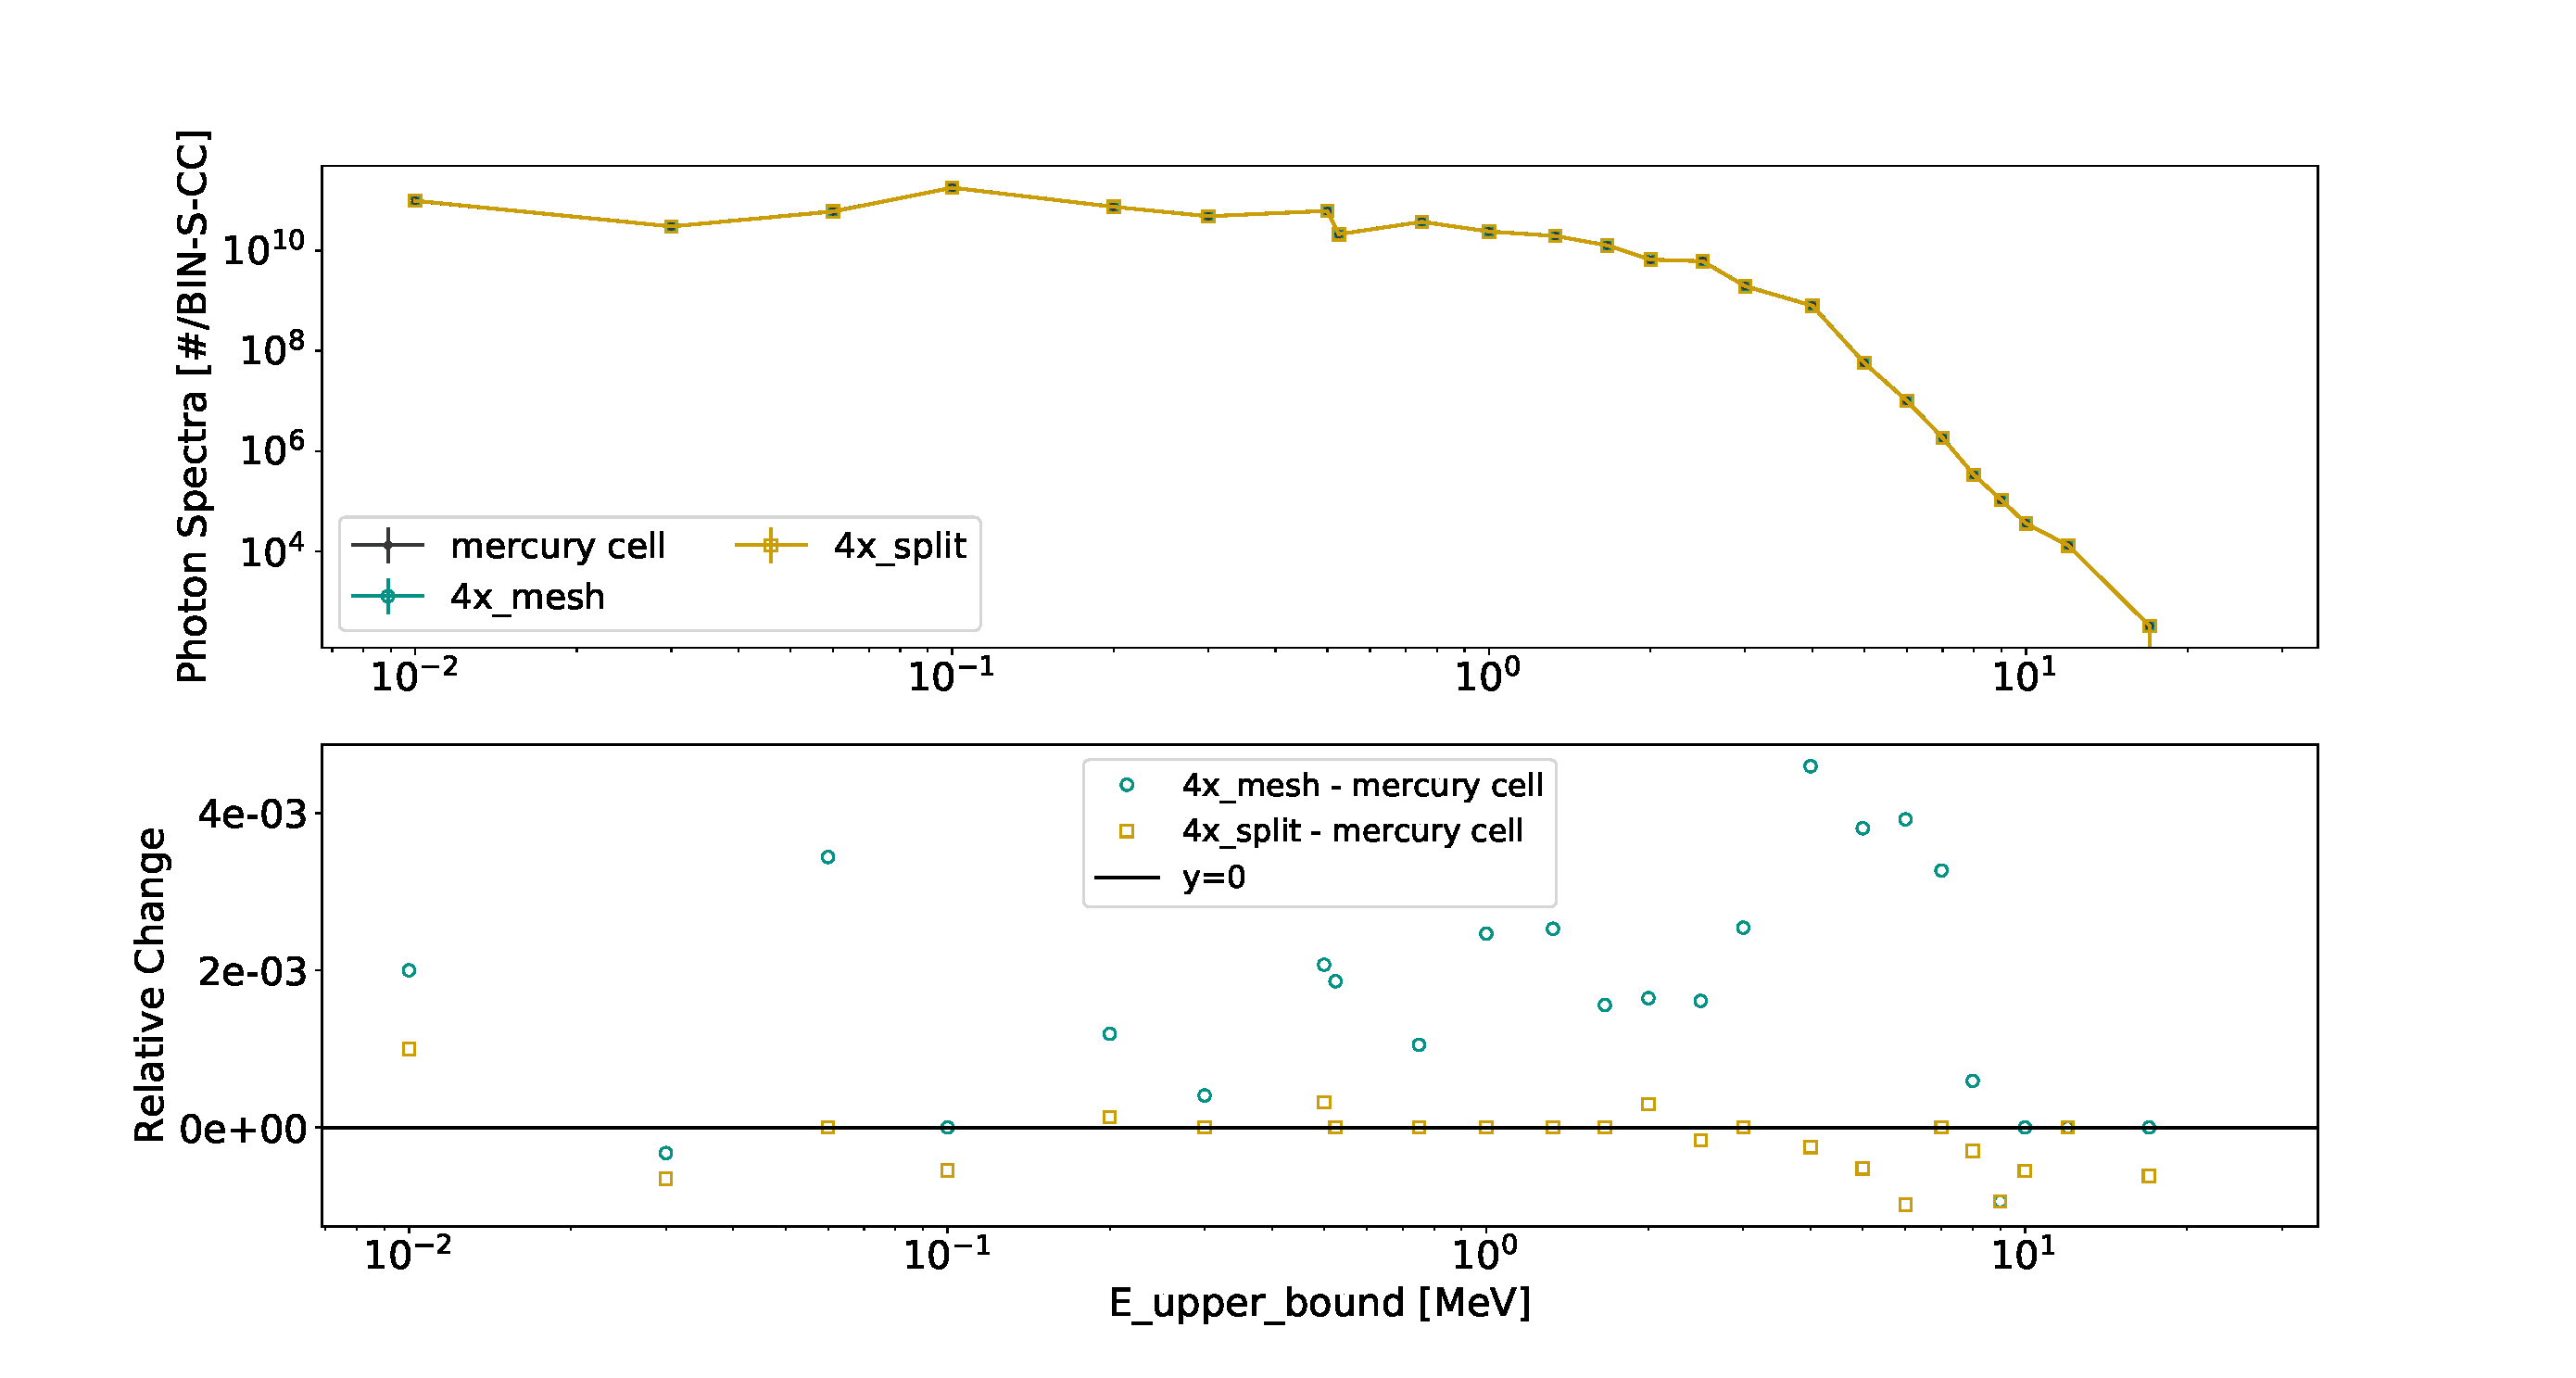
\includegraphics[scale=0.42,trim={3cm 1cm 3cm 3cm},clip]{../figs/toy_p1/spec_VPI_4x.pdf}
 \caption{Photon Spectrum in mercury cell, 4x4x4 mesh, and geometry split}}
 \label{fig:1spec_cell_4x}
\end{figure}



%%%%%%%%%%%%%%%%%%
\newpage
\subsubsection{Verification Problem II}
Similar analysis were done for the second verification problem. Figure
\ref{fig:2prod_cell_1x_2x_4x} show the results collected in the mercury and
steel cell as well as the results for the three meshes. The results for the
mercury and steel cell were added and the results of each voxel in mesh were
added to directly compare the total results.
%
\begin{figure}[h!]
 \centering
 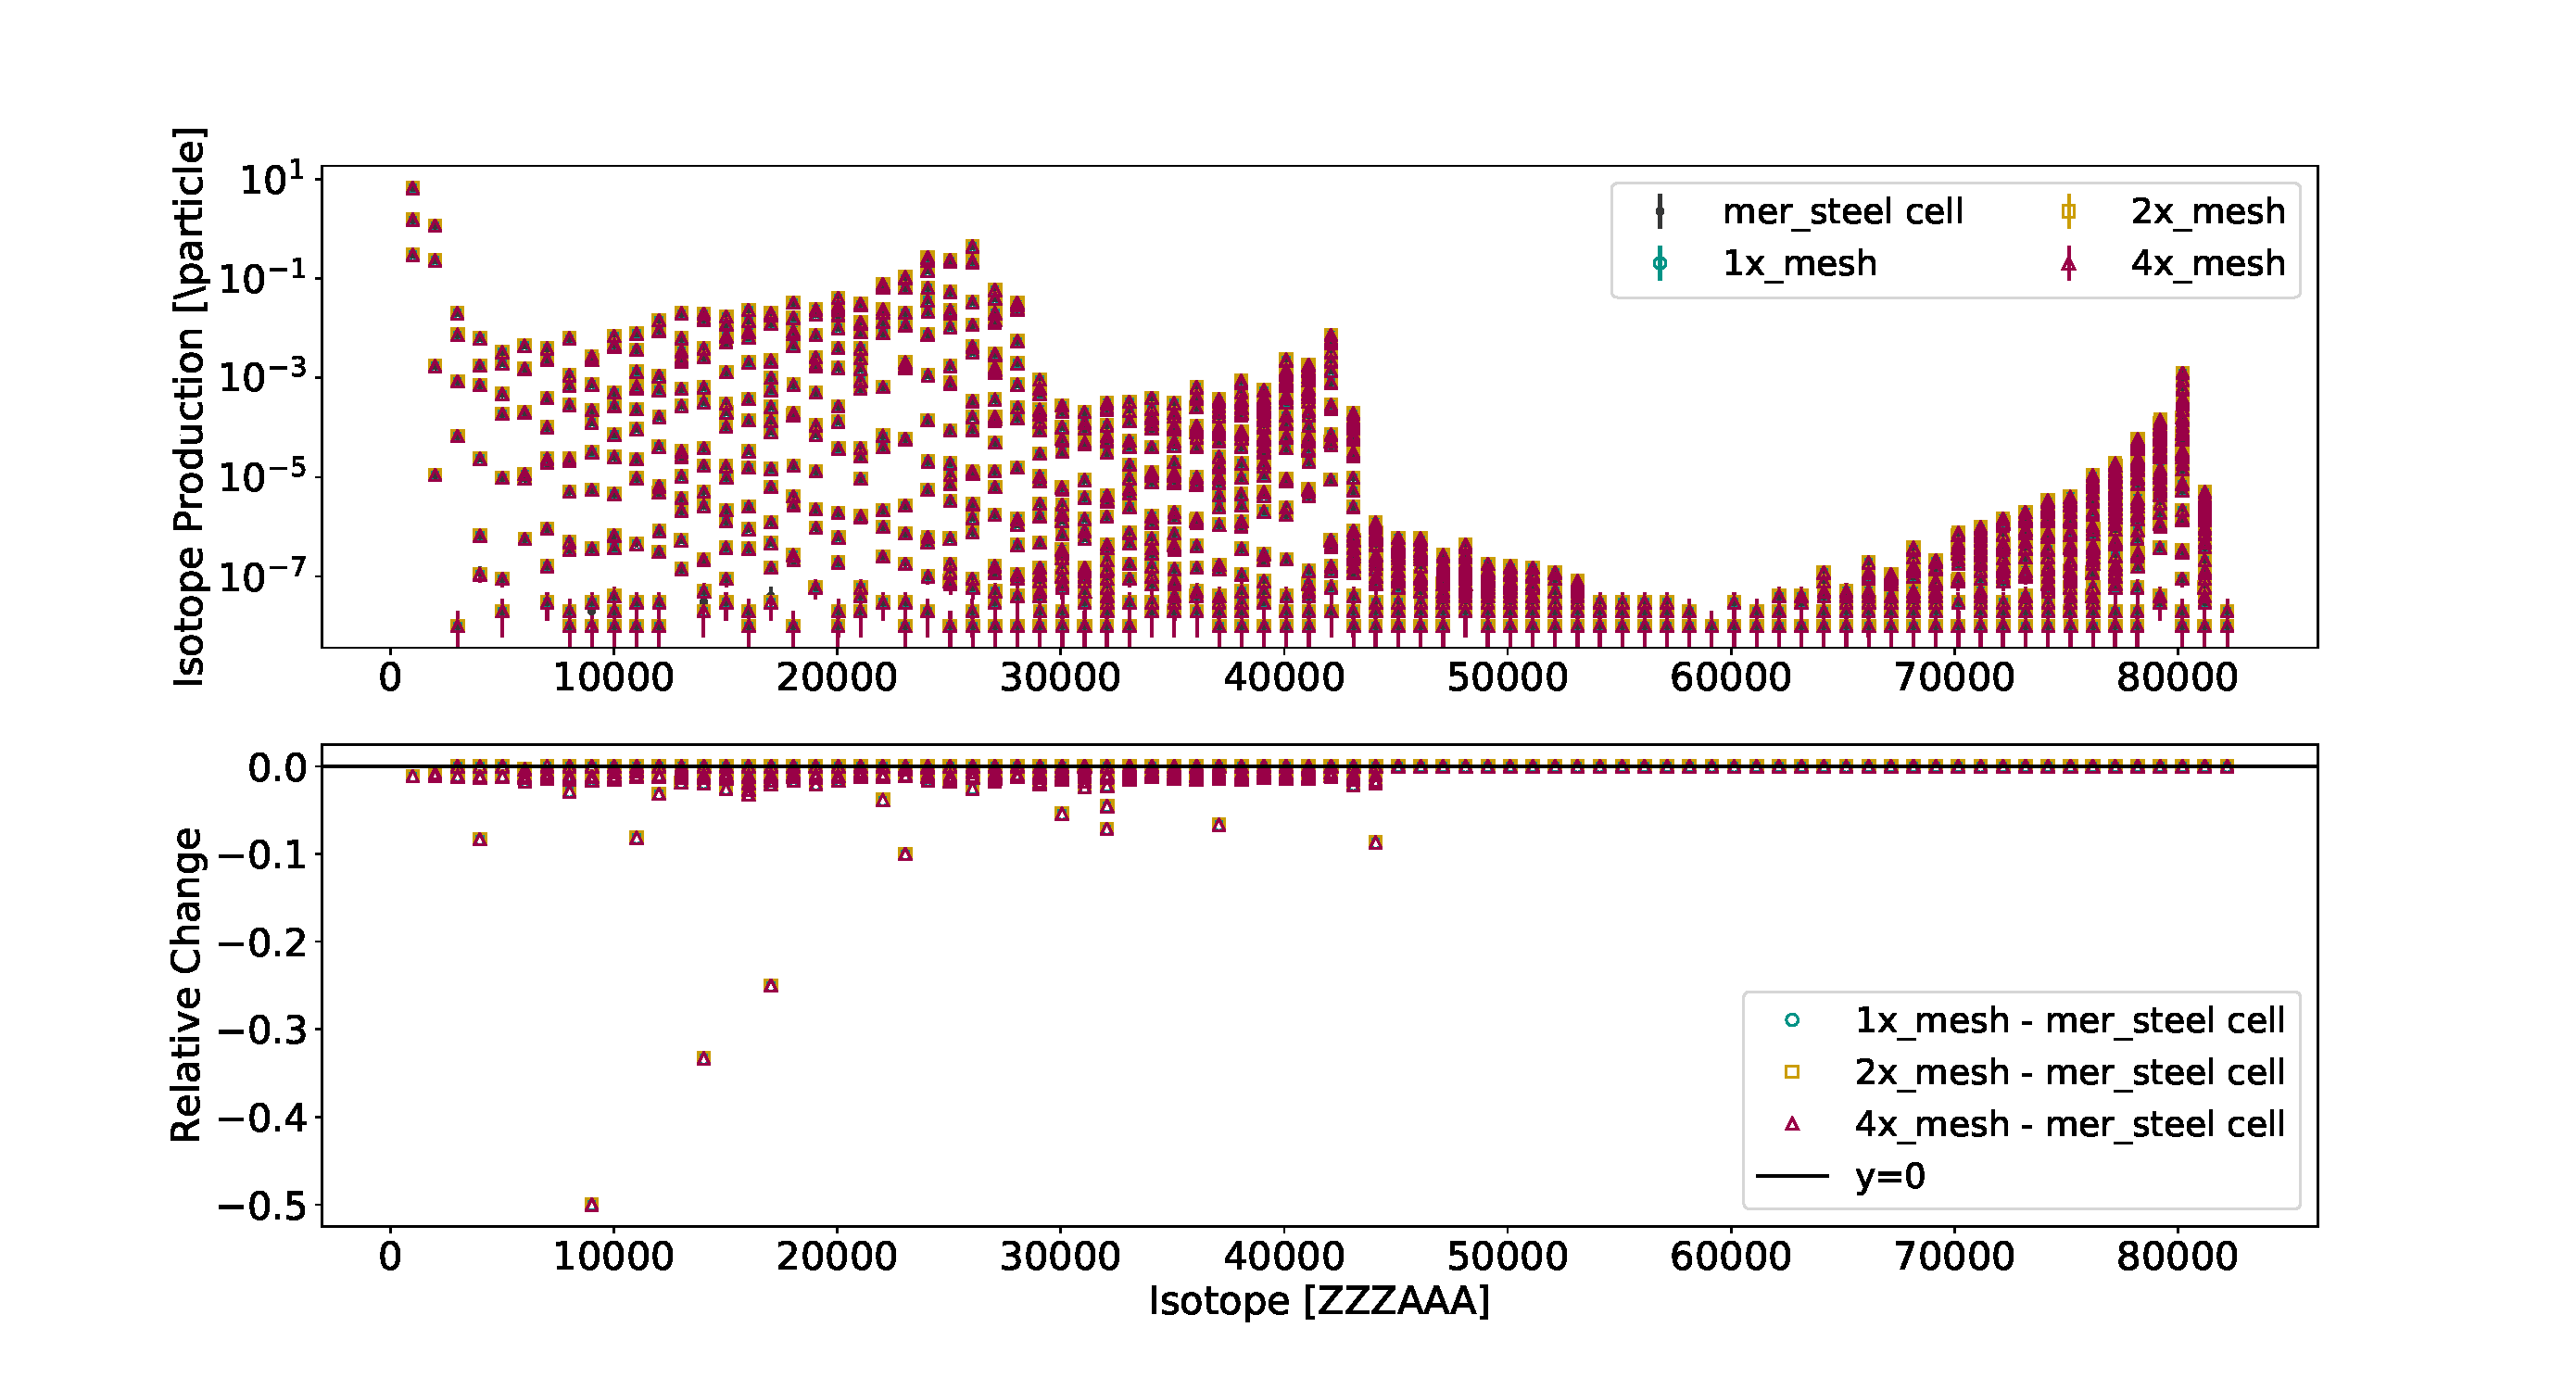
\includegraphics[scale=0.42,trim={2cm 1cm 3cm 2cm},clip]{../figs/toy_p2/prod_VPII_1x_2x_4x.pdf}
 \caption{Radionuclide production for mercury/steel cells and Cartesian meshes}
 \label{fig:2prod_cell_1x_2x_4x}
\end{figure}
%
\\
Figure \ref{fig:2prod_cell_2x} compares the results collected in the geometric
cell, the summed up results of the 2x2x2 mesh and the 2x2x2 divided geometry.
%
\begin{figure}[h!]
 \centering
 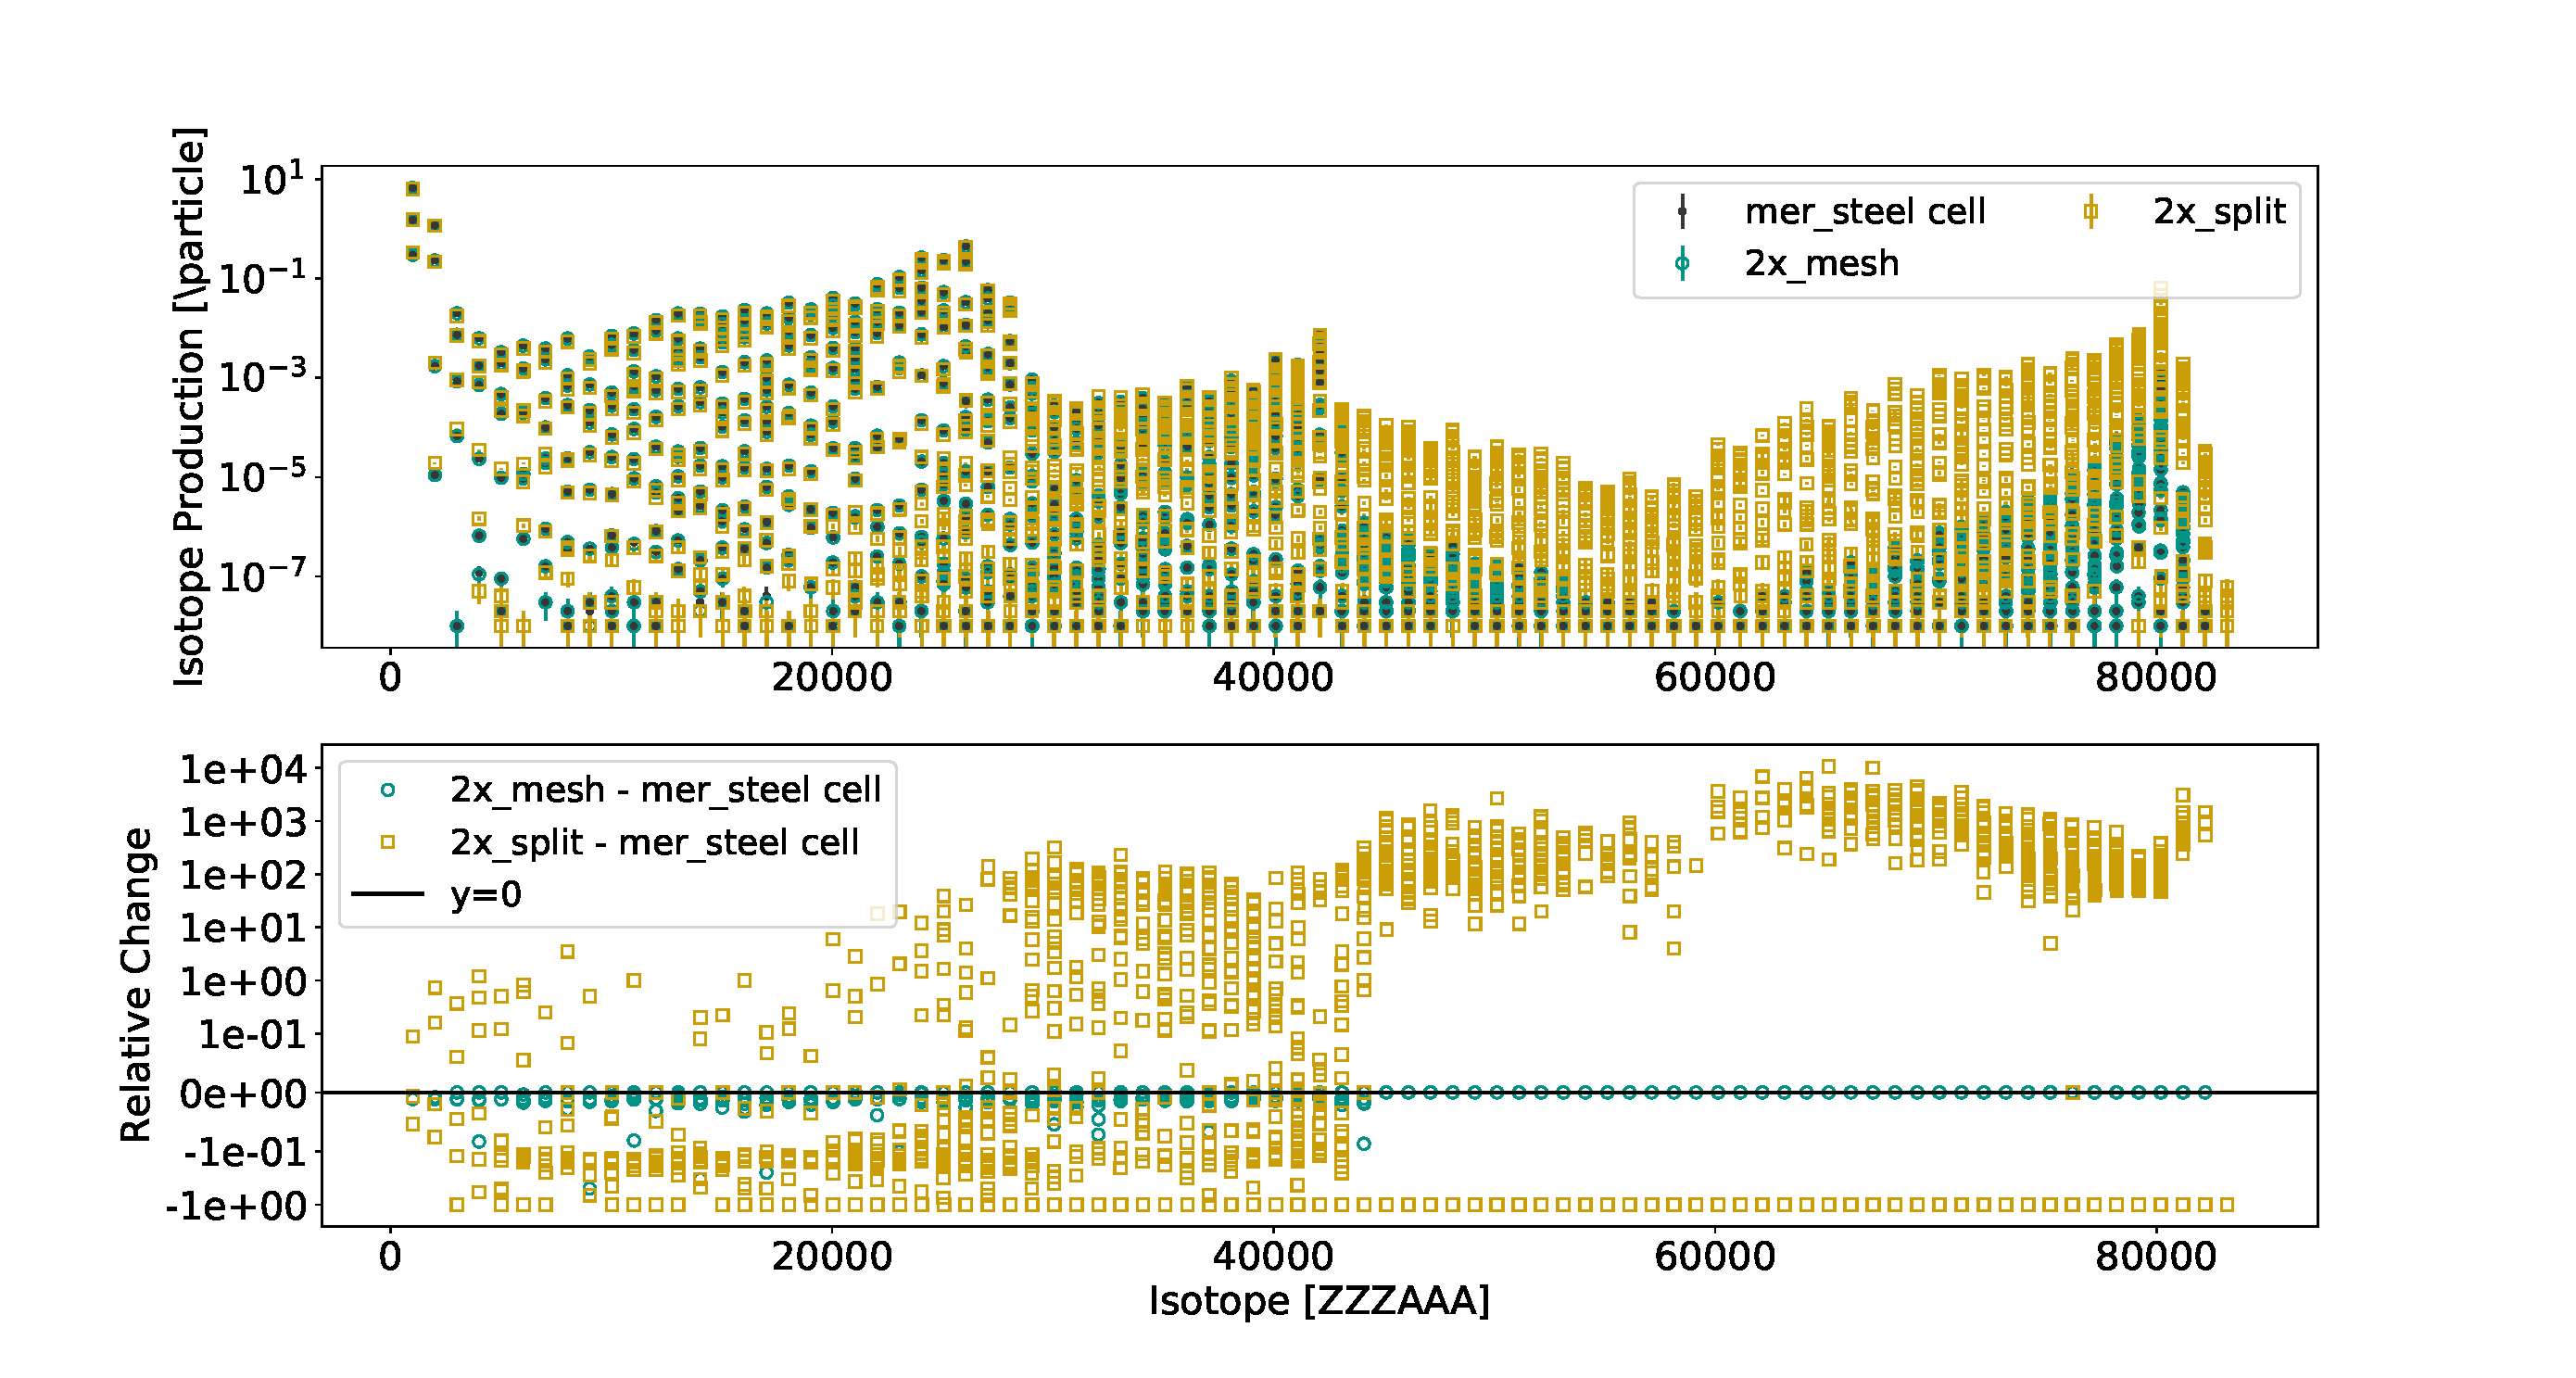
\includegraphics[scale=0.42,trim={3cm 1cm 3cm 3cm},clip]{../figs/toy_p2/prod_VPII_2x.pdf}
 \caption{Radionuclide production mercury/steel cells, 2x2x2 mesh, and 2x2x2 divided geometry}
 \label{fig:2prod_cell_2x}
\end{figure}
%
\\
A similar comparison was made for the 4x4x4 mesh and the 4x4x4 divided geometry
which can be seen in Figure \ref{fig:2prod_cell_4x}
%
\begin{figure}[h!]
 \centering
 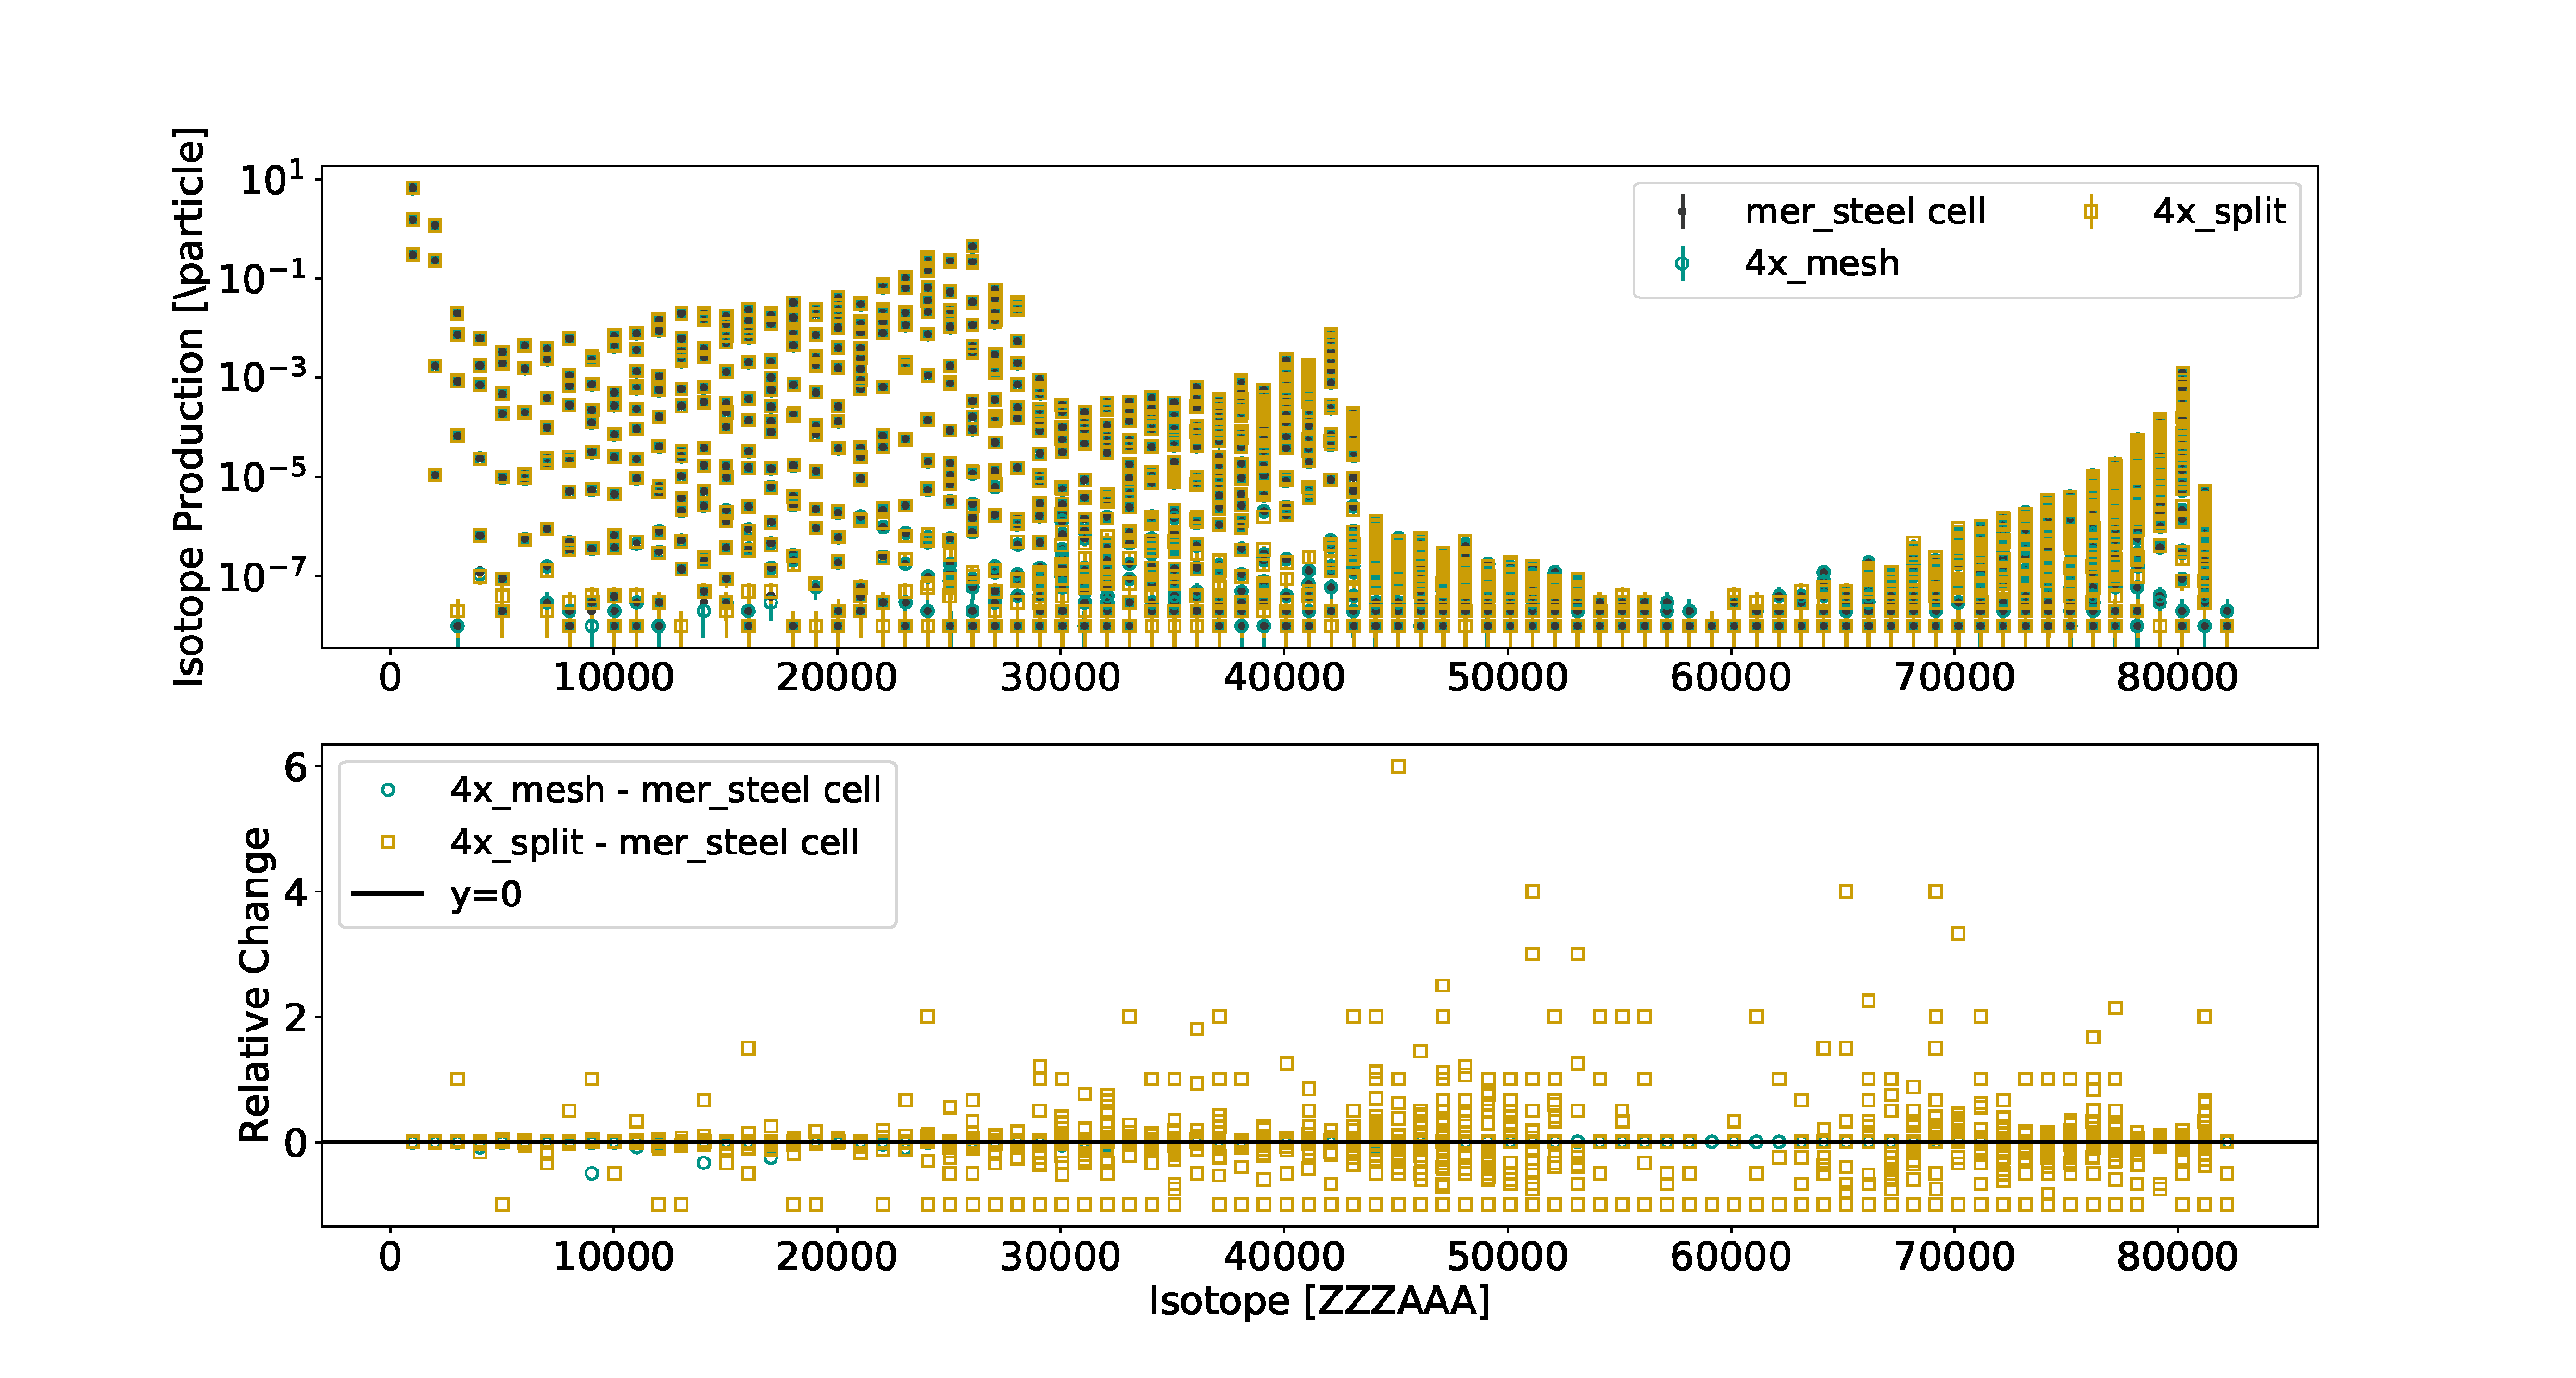
\includegraphics[scale=0.42,trim={3cm 1cm 3cm 3cm},clip]{../figs/toy_p2/prod_VPII_4x.pdf}
 \caption{Radionuclide production for mercury/steel cells, 4x4x4 mesh, and 4x4x4 divided geometry}
 \label{fig:2prod_cell_4x}
\end{figure}
%
\\
Figure \ref{fig:2prod_cell_1x_2x_4x} shows most nuclides have a small relative
change. There are a few nuclides that greater than 10\percent relative change.
Figure \ref{fig:2prod_cell_2x} shows that many nuclides resulting from the
divided geometry have extremely high relative change. This is largely due to
having to mix the mercury and steel materials in the neutron transport. Lastly
Figure \ref{fig:2prod_cell_4x} shows results similar to the results obtained in
the first verification problem.
%
\begin{figure}[h!]
 \centering
 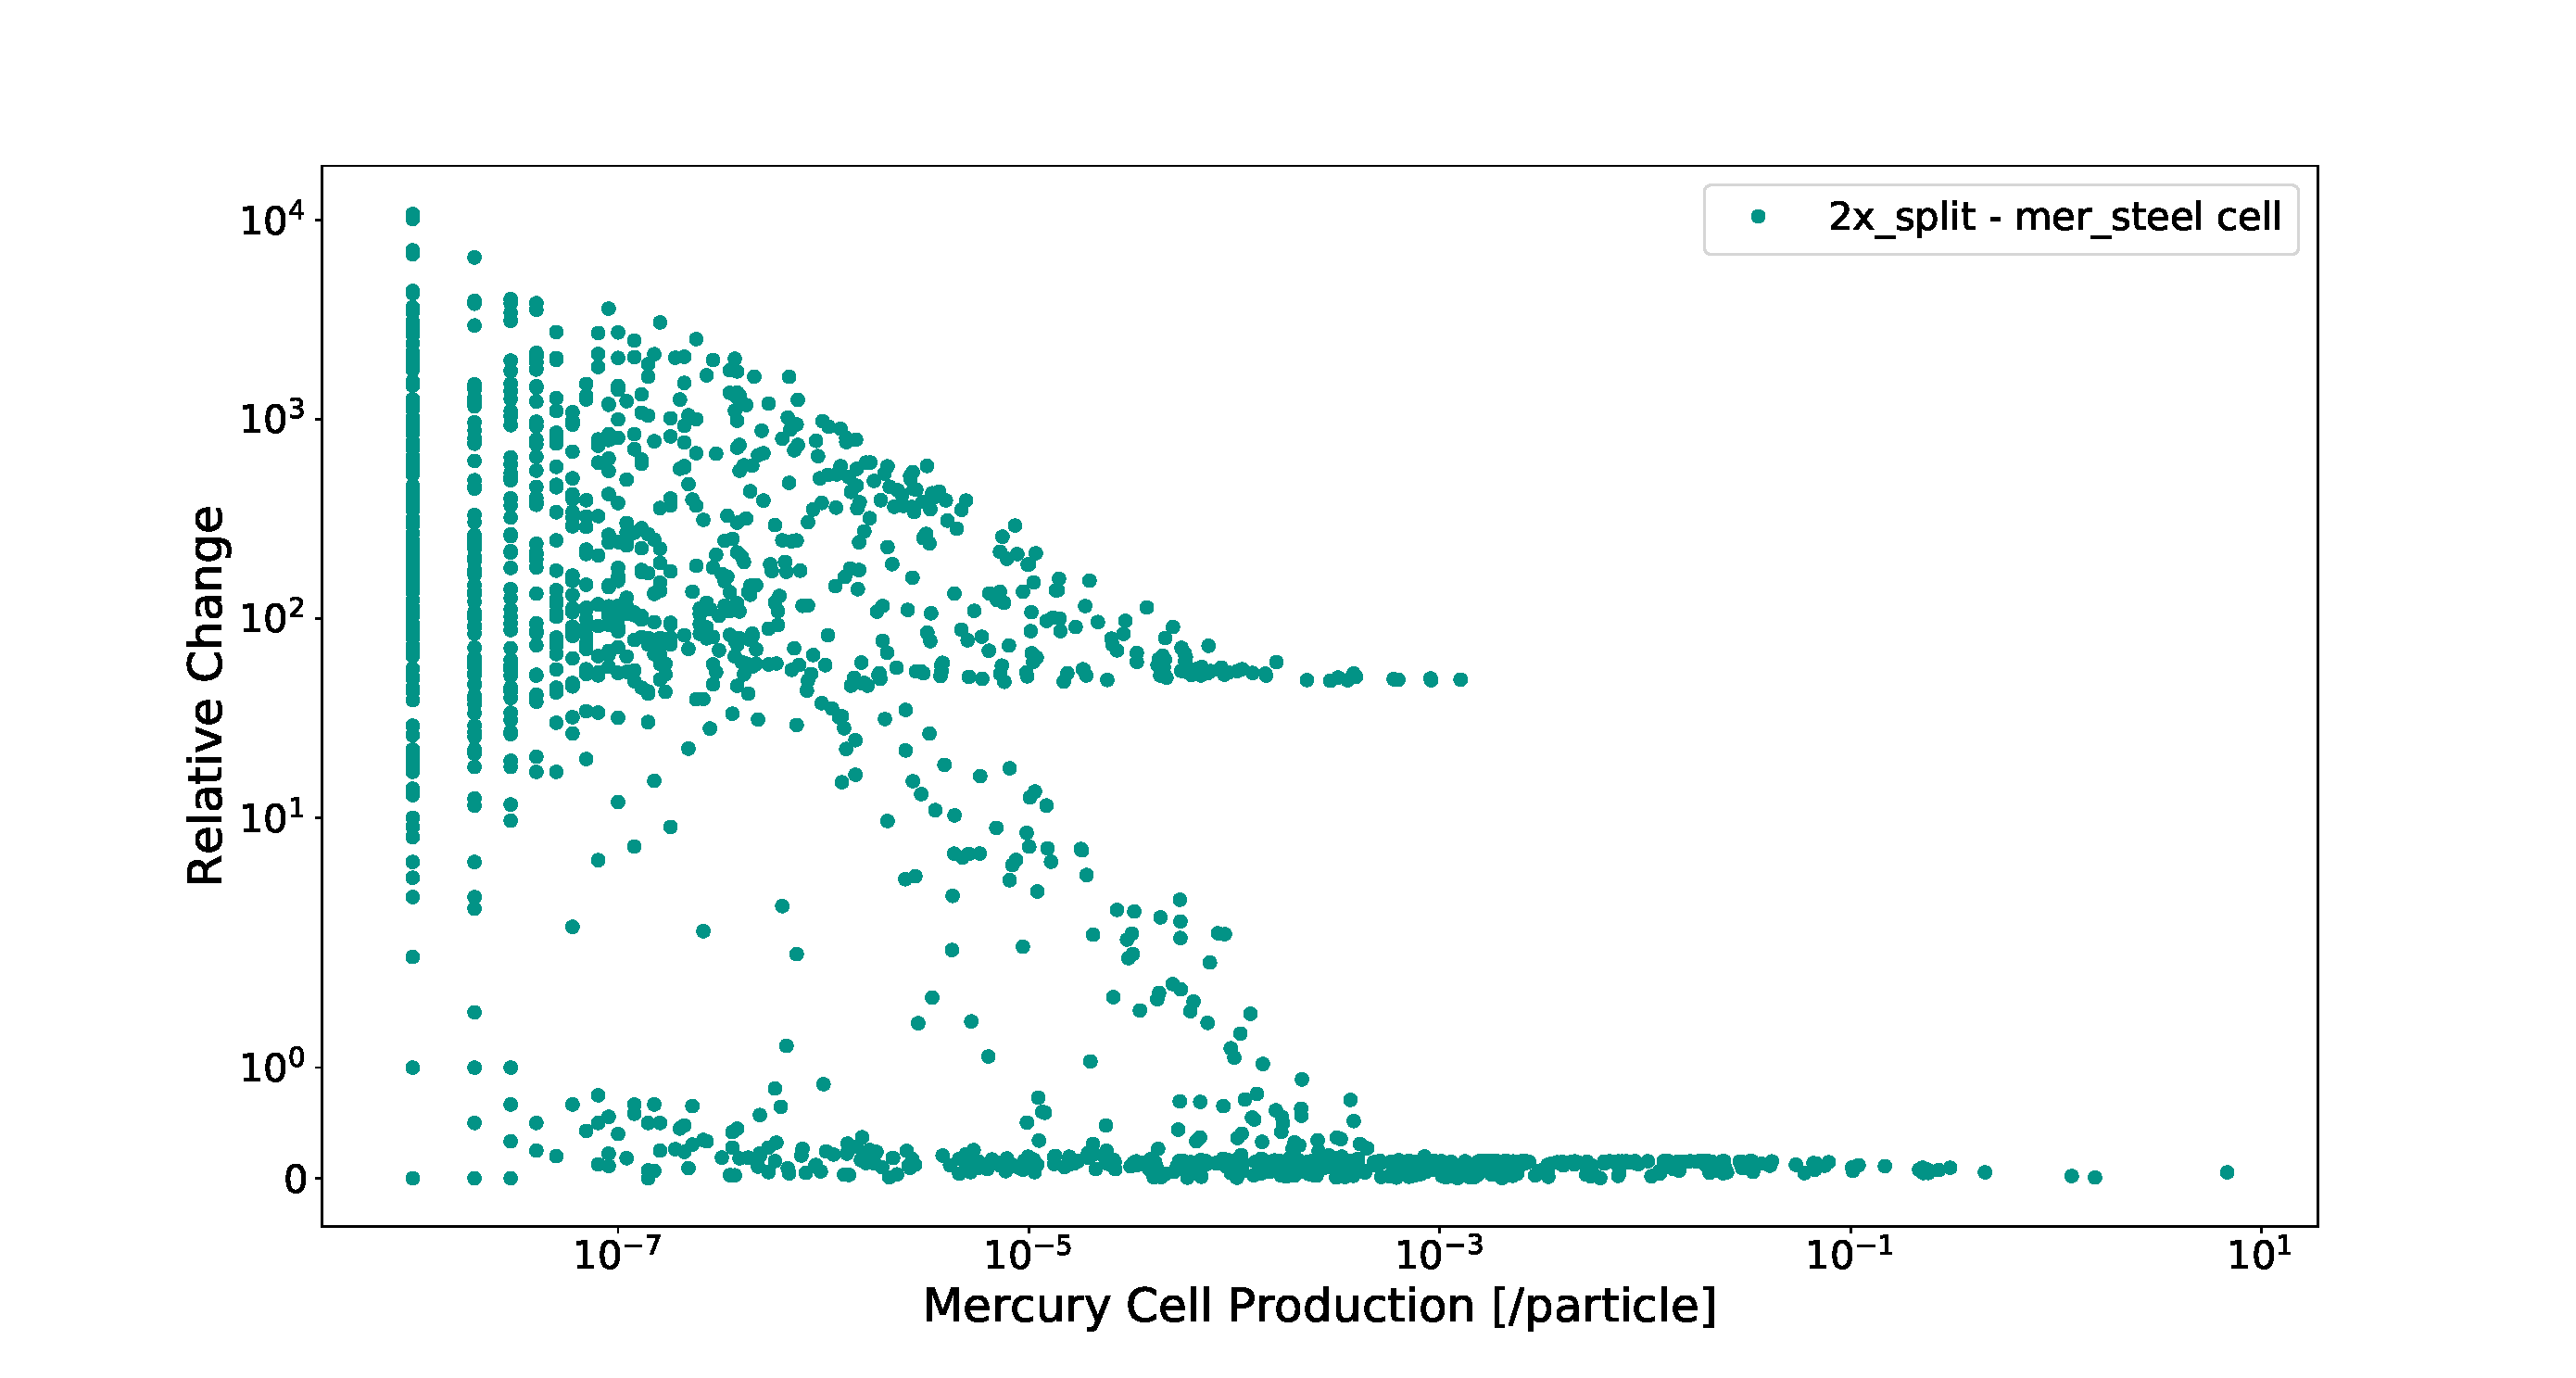
\includegraphics[scale=0.42,trim={3cm 0.5cm 3cm 3cm},clip]{../figs/toy_p2/prod_VPII_rc_2x_split.pdf}
 \caption{Relative change between cell method and 2x2x2 geometry split vs. the isotope production of the mercury cell}
 \label{fig:2prod_cell_2x_rc}
\end{figure}
\begin{figure}[h!]
 \centering
 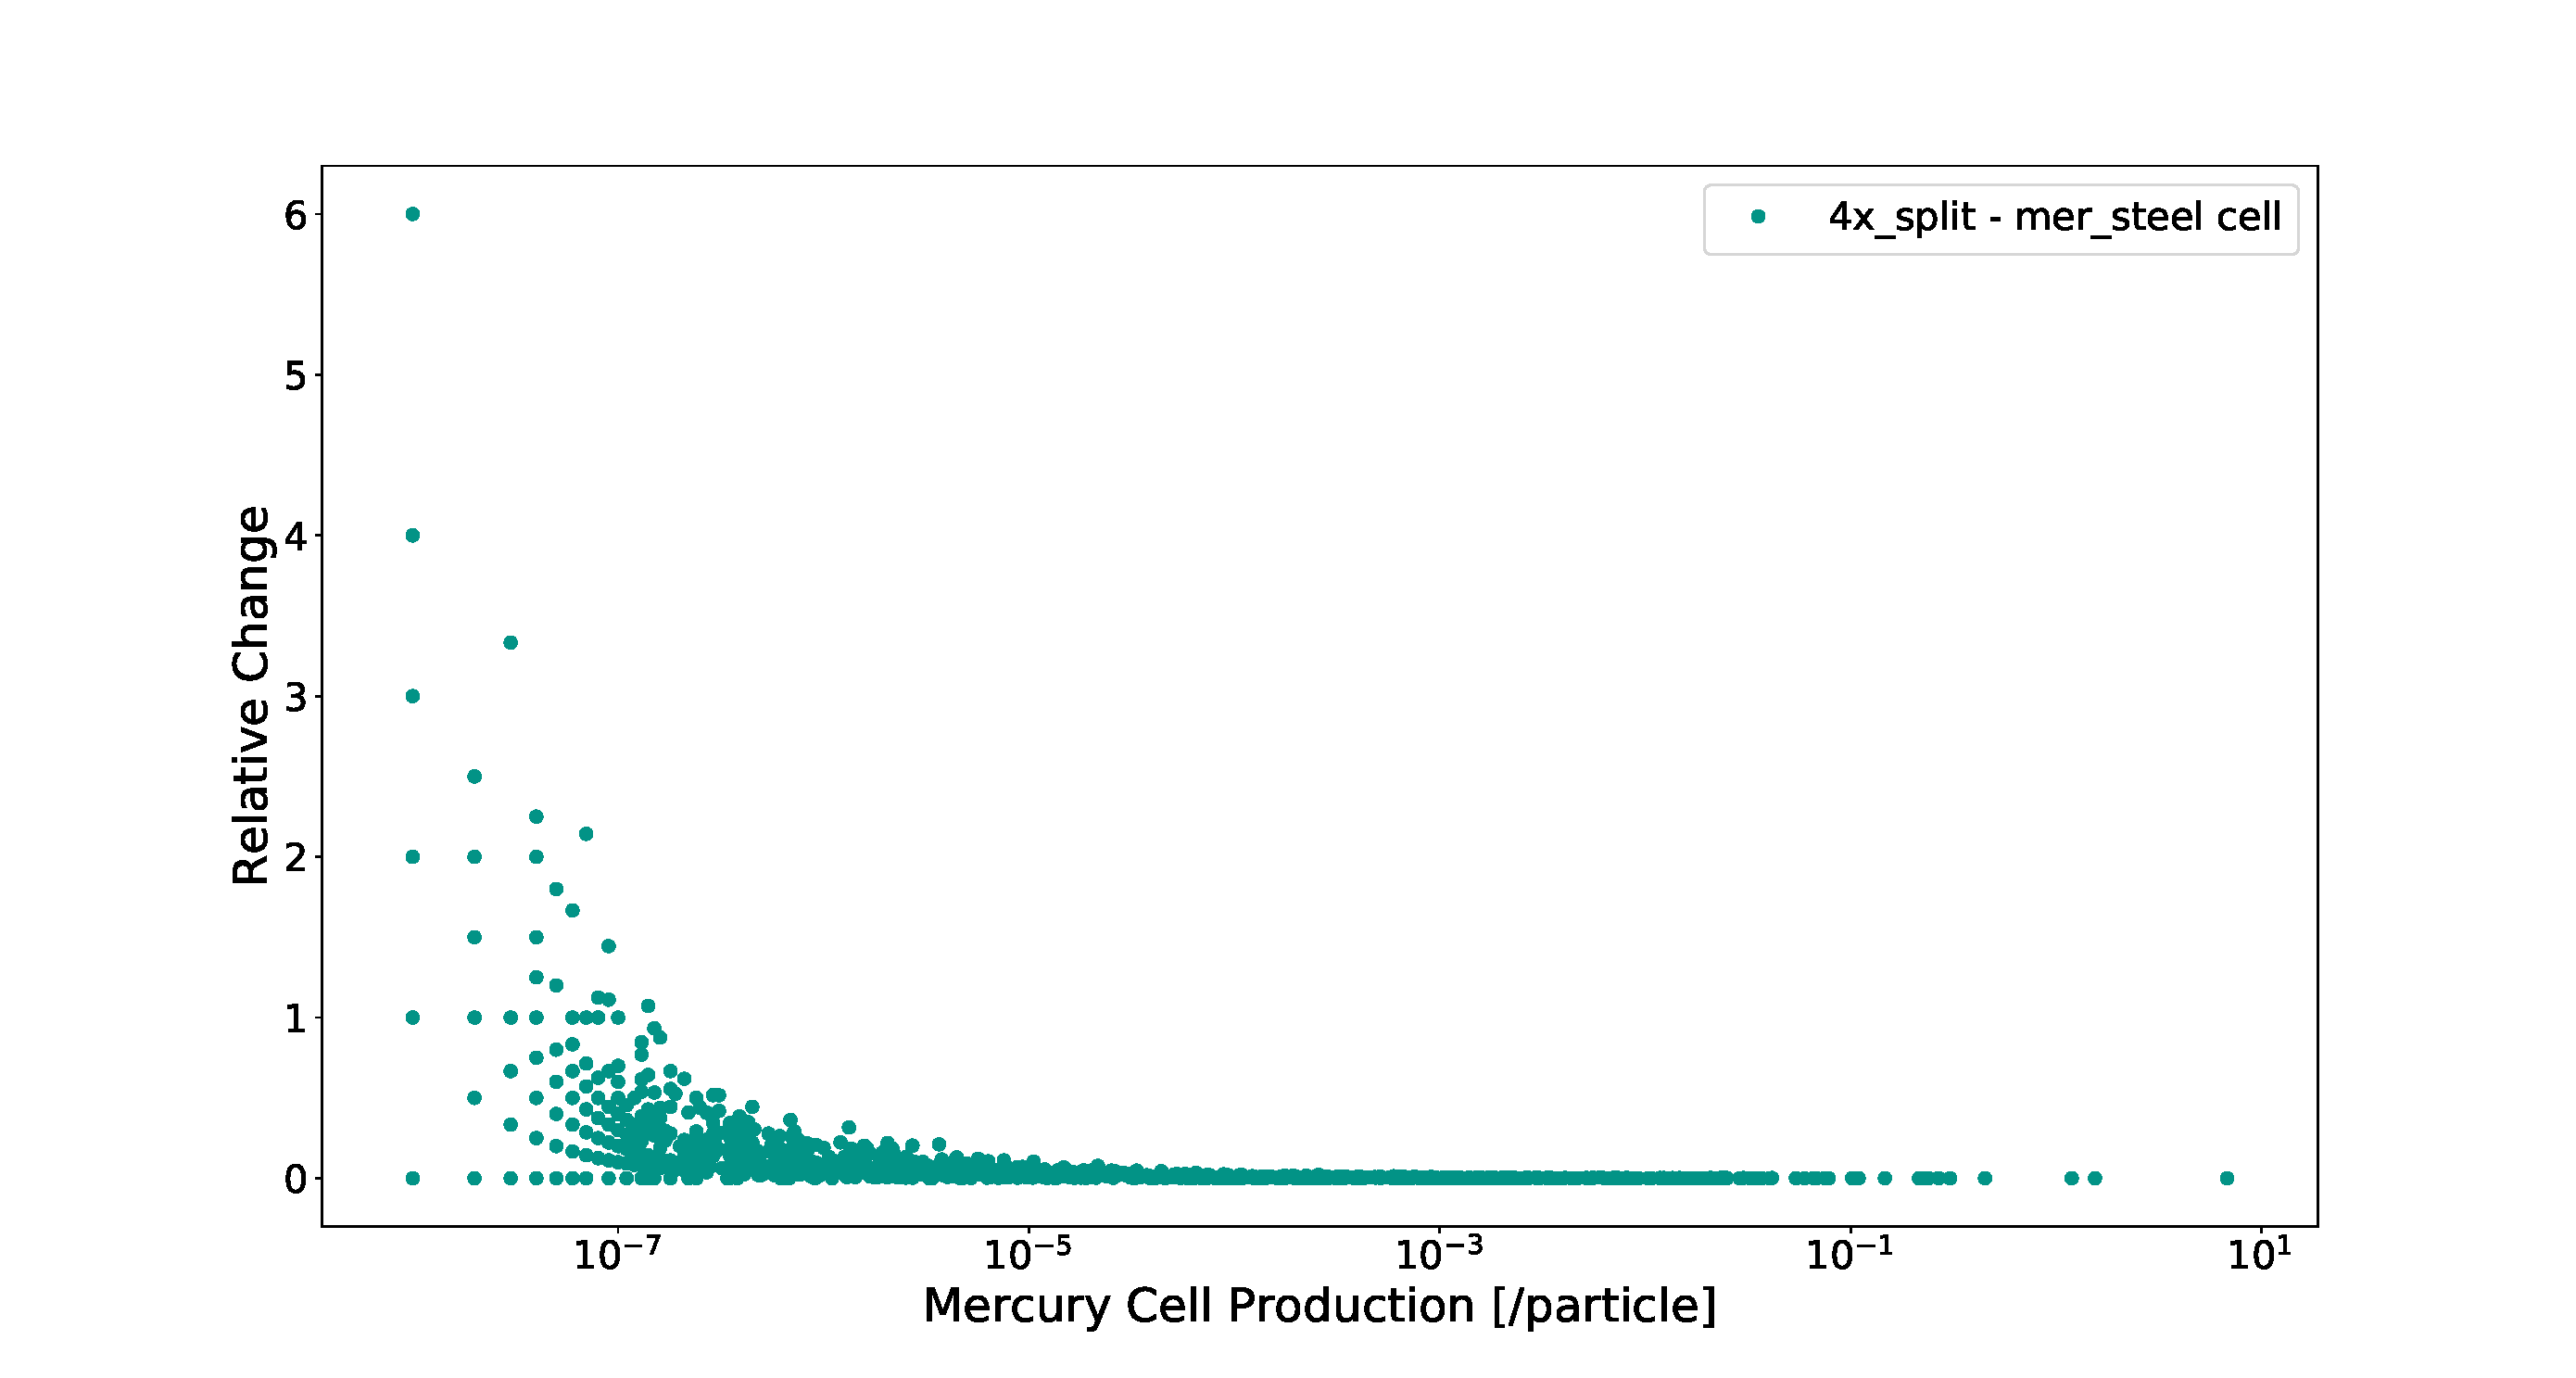
\includegraphics[scale=0.42,trim={3cm 0.5cm 3cm 3cm},clip]{../figs/toy_p2/prod_VPII_rc_4x_split.pdf}
 \caption{Relative change between cells and 4x4x4 geometry split vs. the isotope production of the mercury cell}
 \label{fig:2prod_cell_4x_rc}
\end{figure}
%

\begin{figure}[h!]
 \centering
 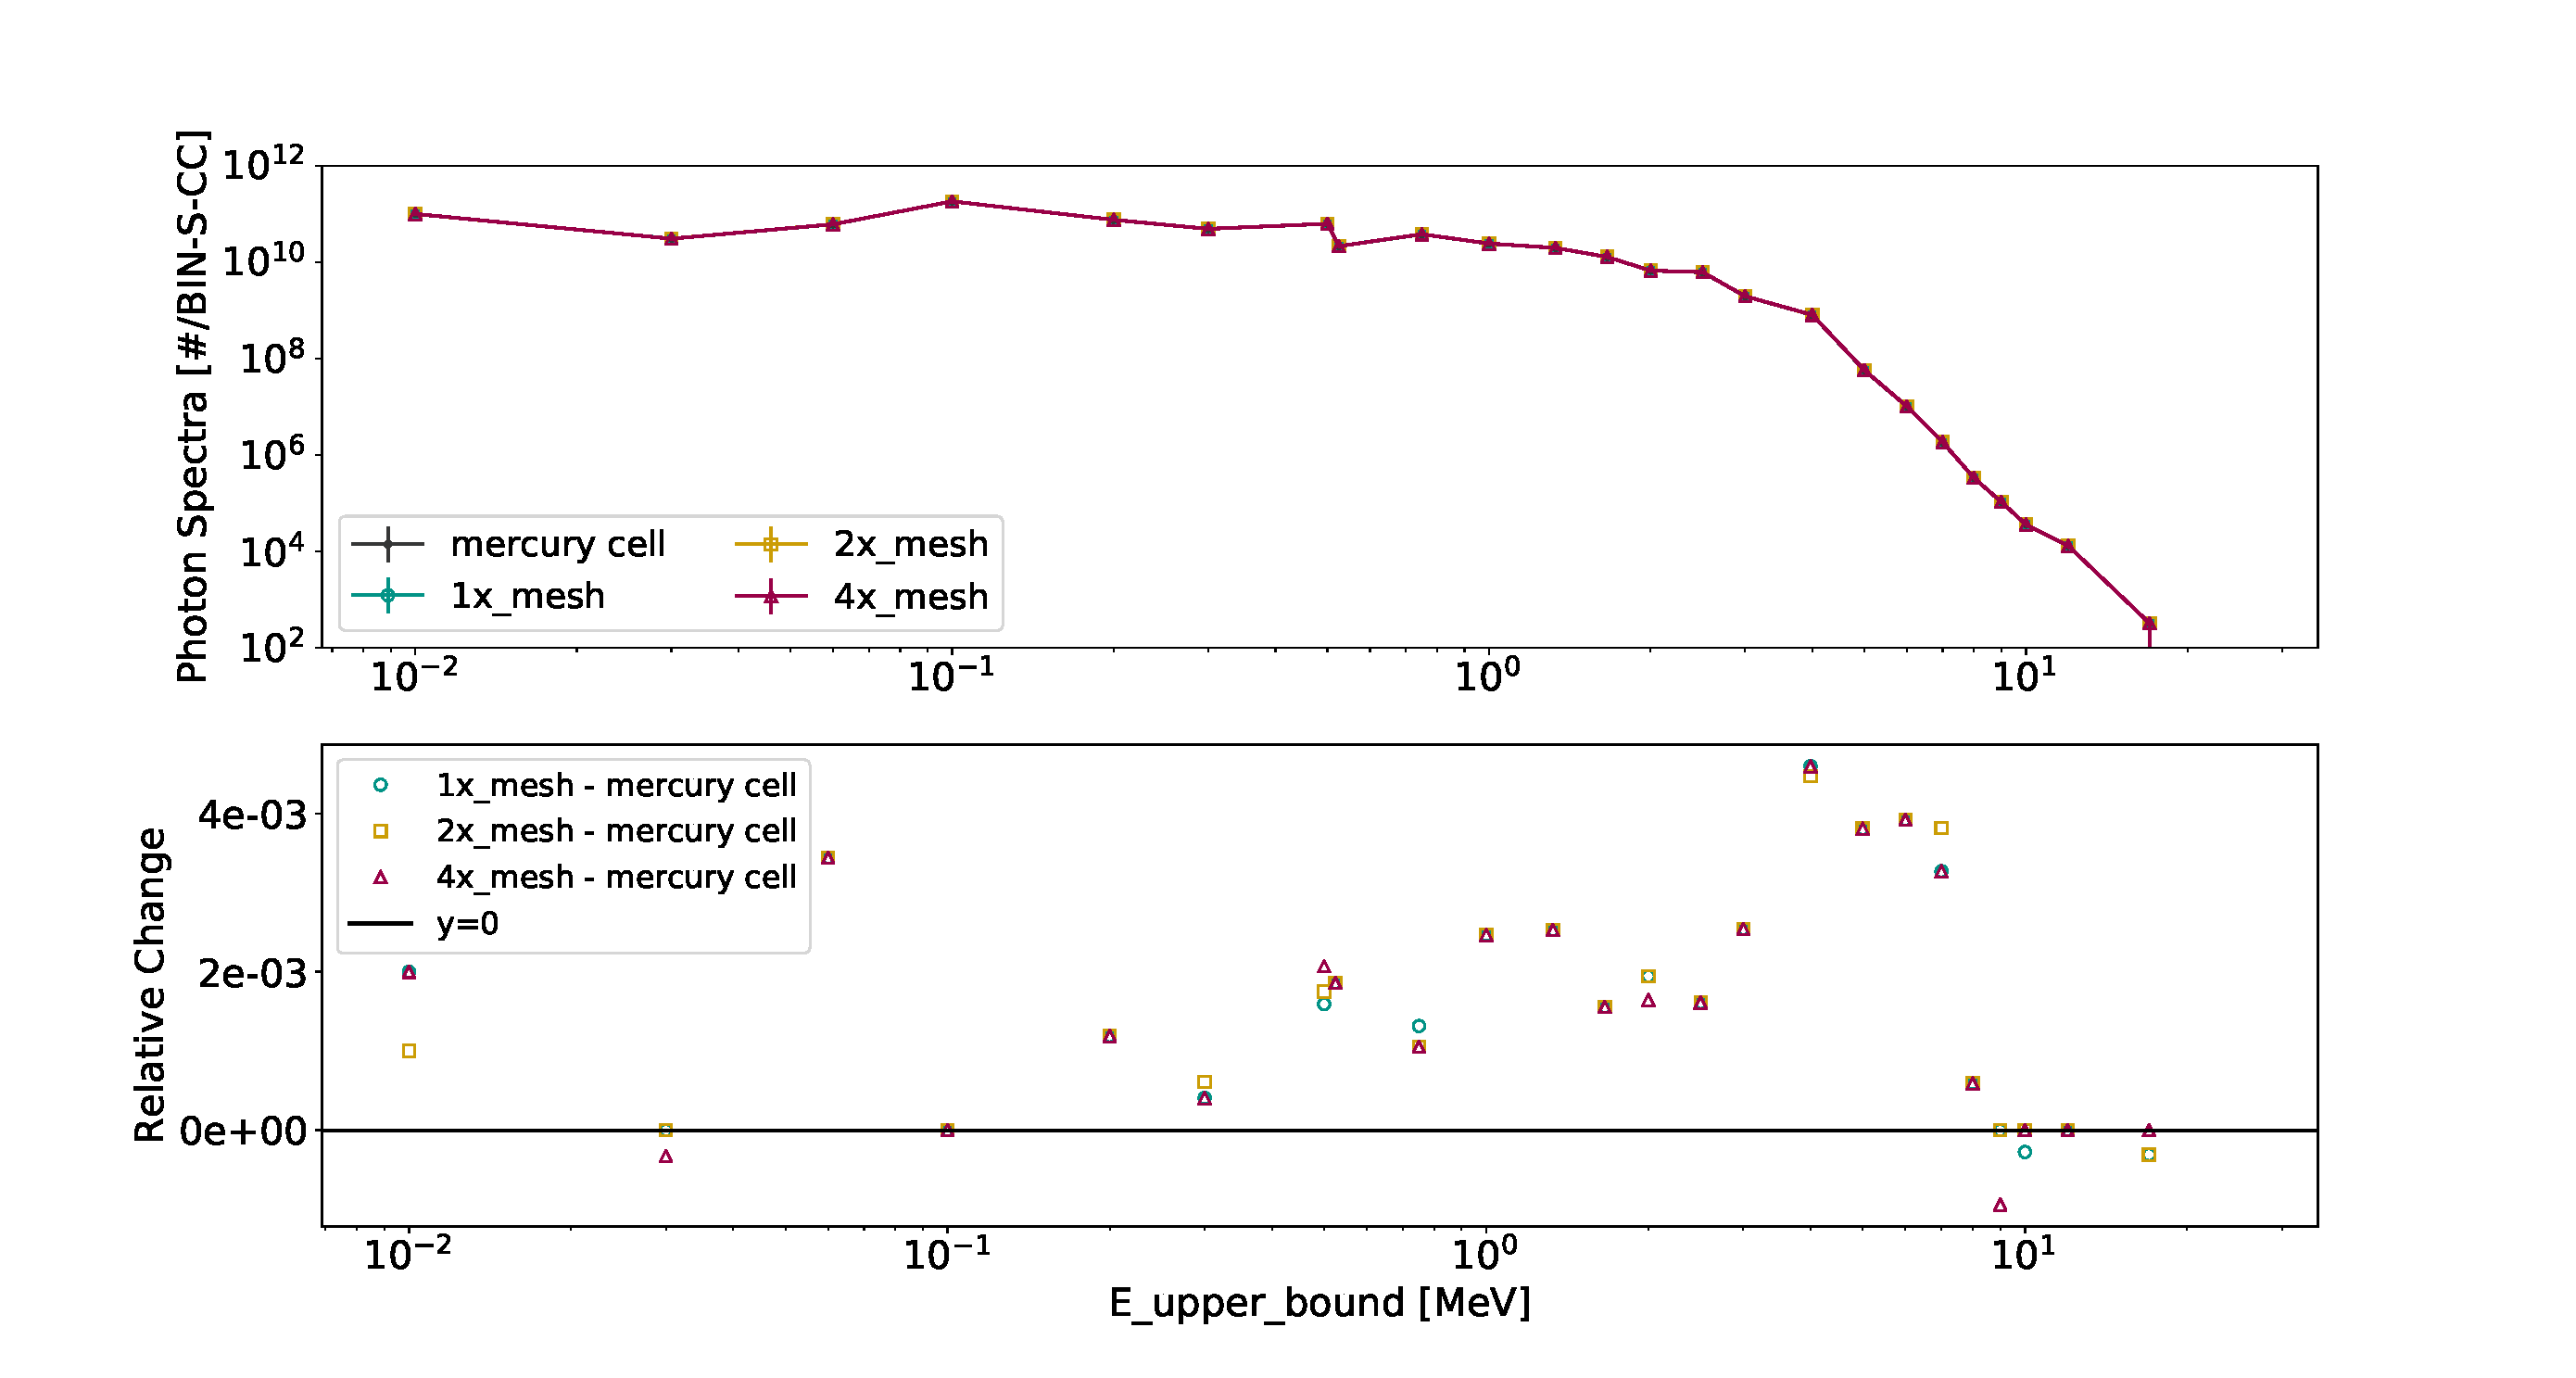
\includegraphics[scale=0.42,trim={2cm 0.5cm 3cm 2cm},clip]{../figs/toy_p1/spec_VPI_1x_2x_4x.pdf}
 \caption{Photon Spectrum in mercury cell and different meshes}
 \label{fig:1spec_cell_1x_2x_4x}
\end{figure}
%
A comparison between the results in the mesh and the split geometry can be seen
in Figure \ref{fig:1spec_cell_2x} and \ref{fig:1spec_cell_4x}.
%
\begin{figure}[h!]
 \centering
 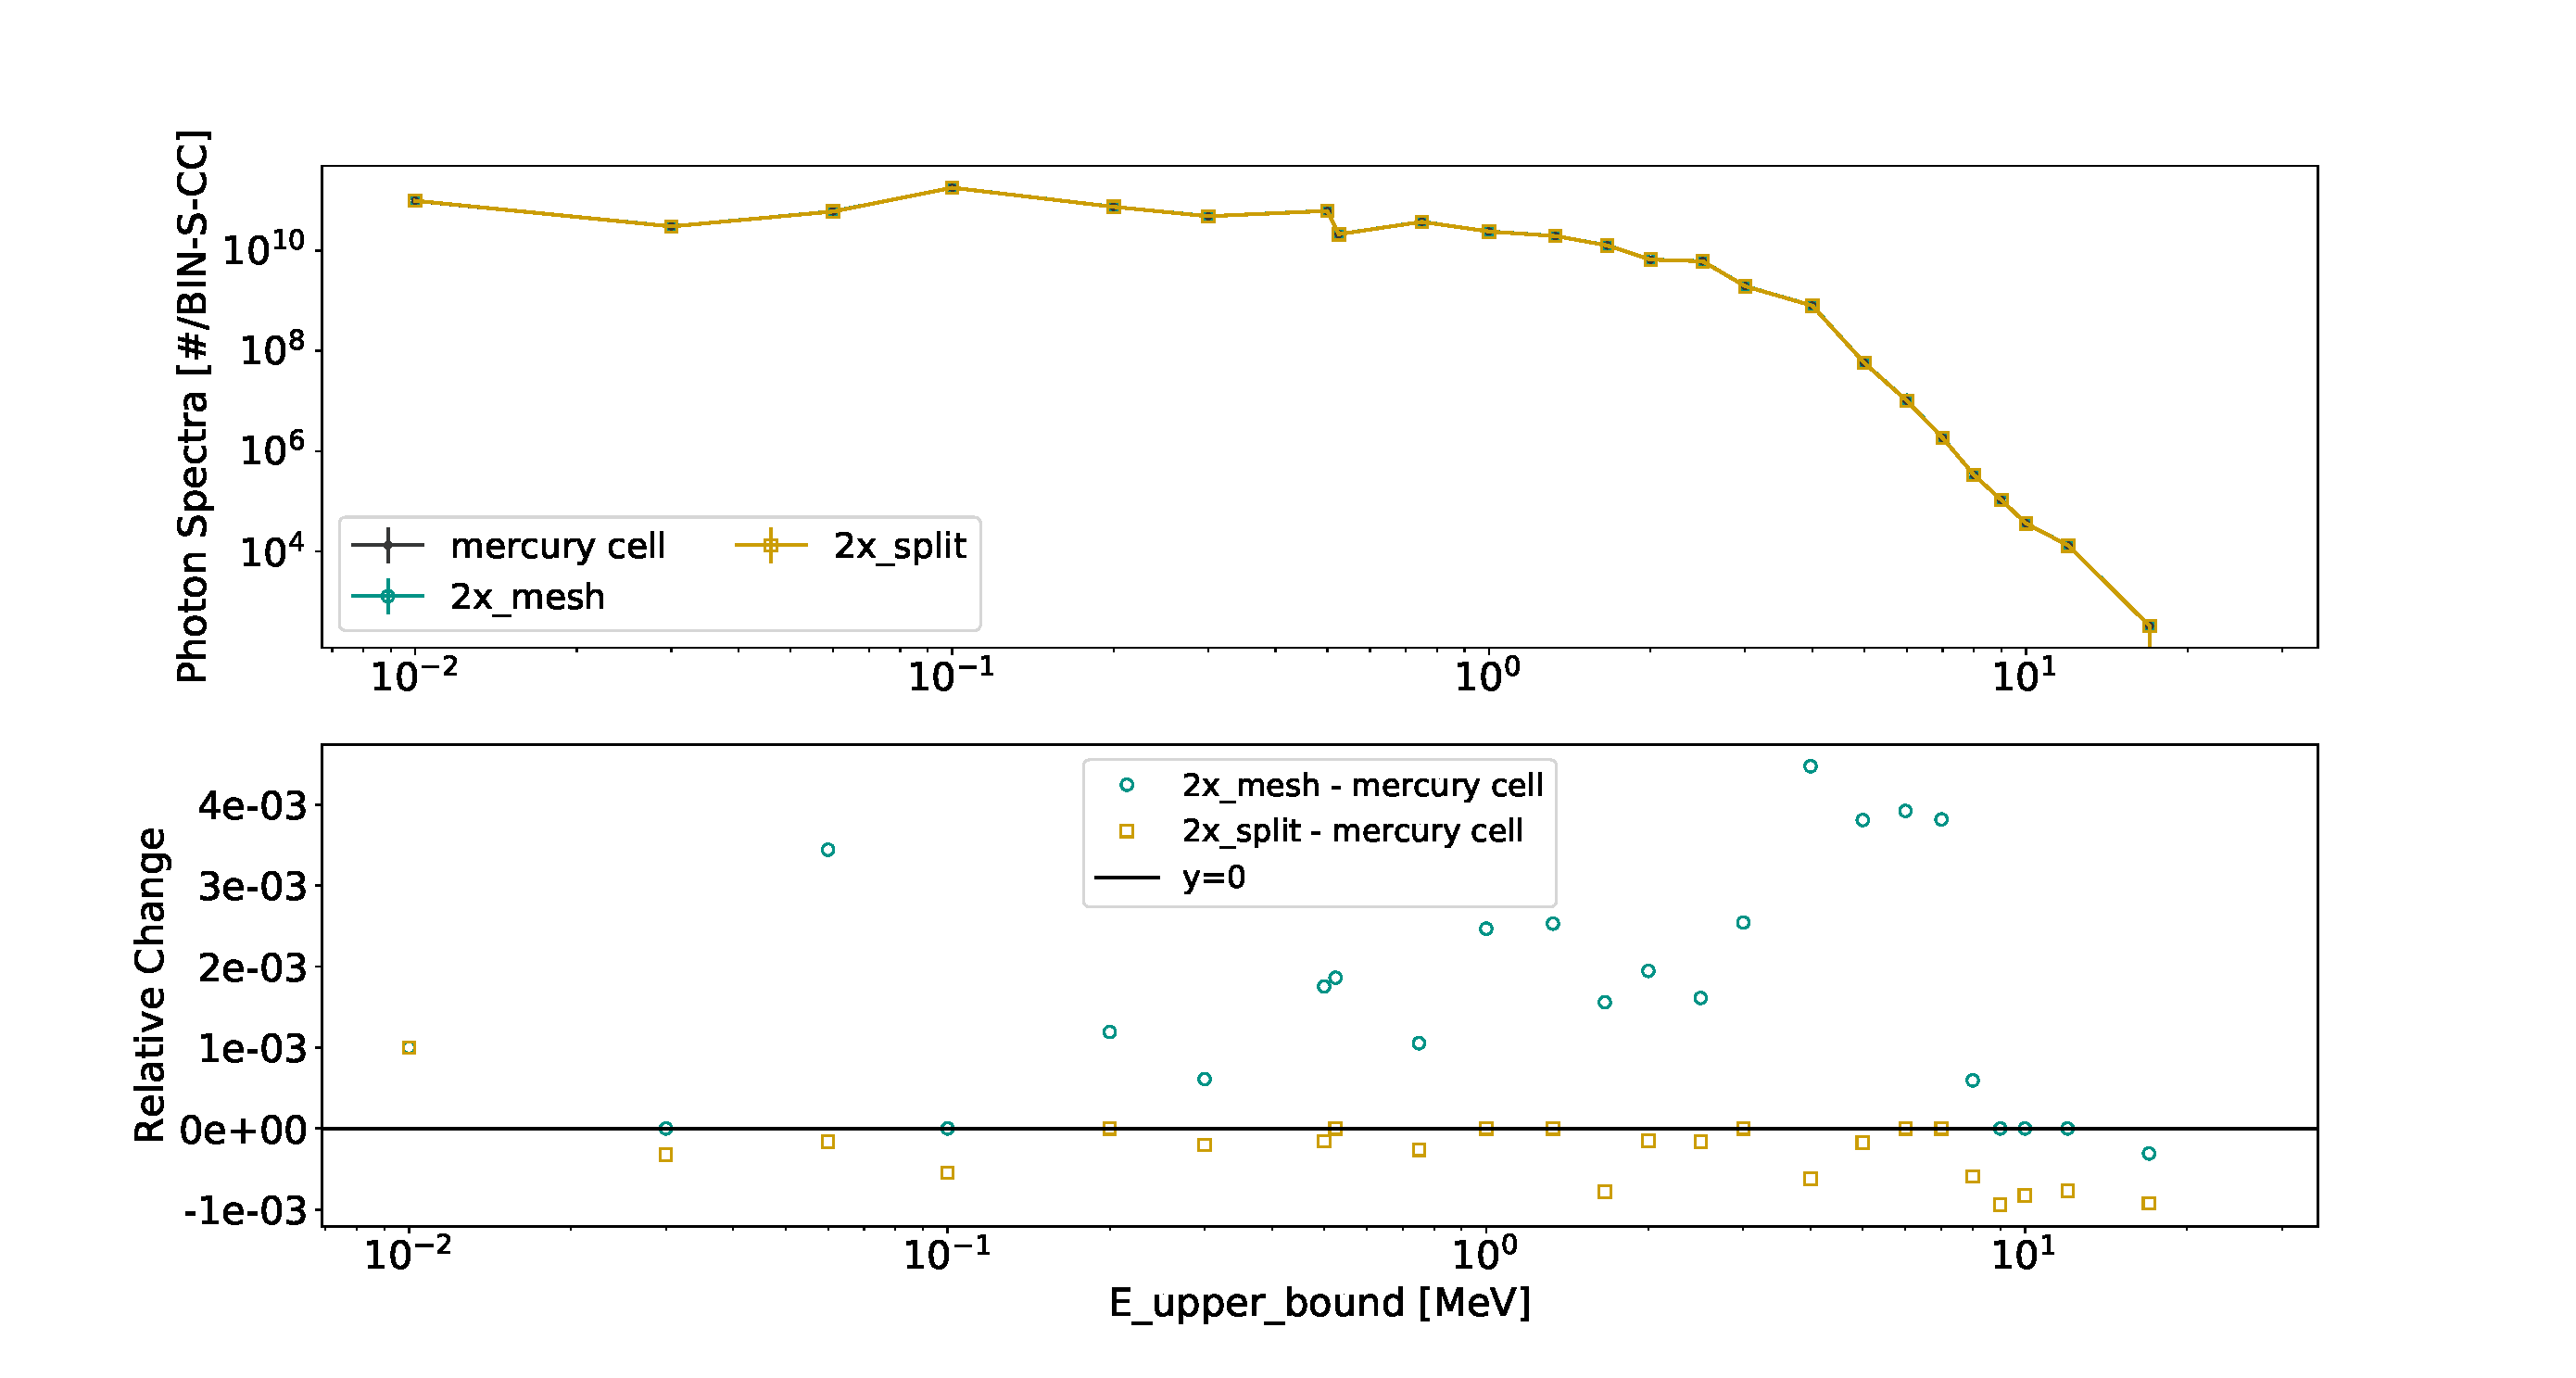
\includegraphics[scale=0.42,trim={3cm 1cm 3cm 3cm},clip]{../figs/toy_p1/spec_VPI_2x.pdf}
 \caption{Photon Spectrum in mercury cell, 2x2x2 mesh, and geometry split}
 \label{fig:1spec_cell_2x}
\end{figure}
\begin{figure}[h!]
 \centering
 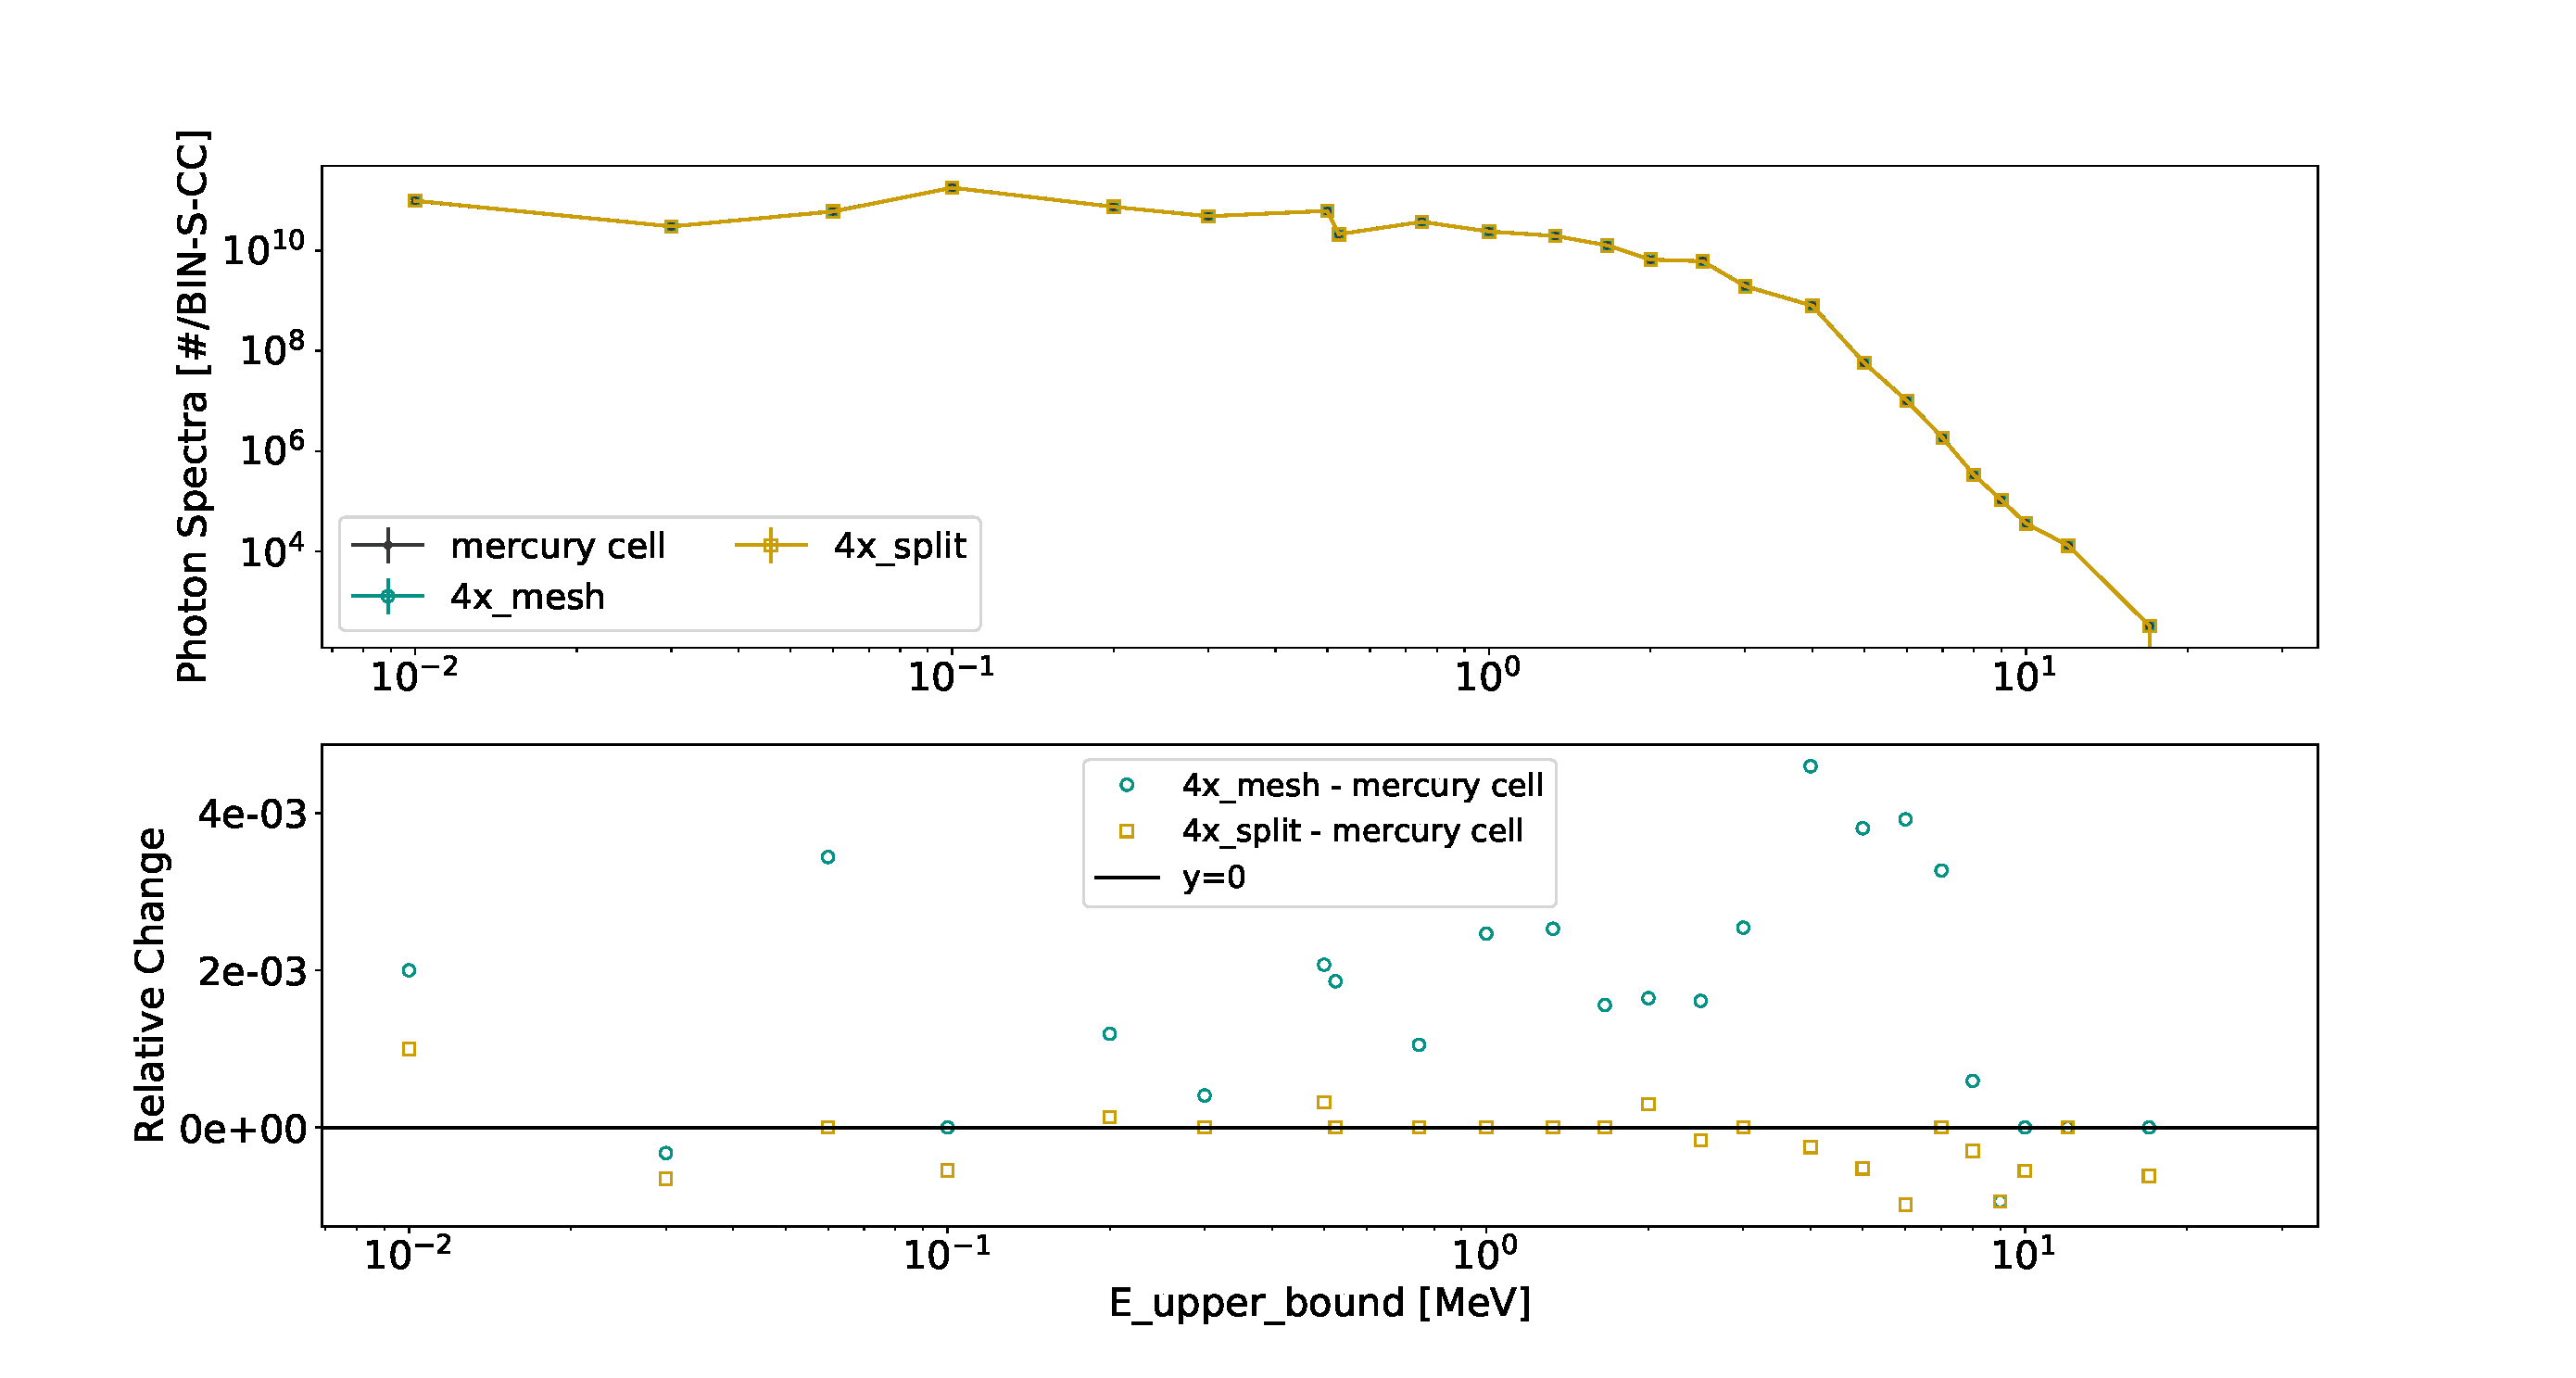
\includegraphics[scale=0.42,trim={3cm 1cm 3cm 3cm},clip]{../figs/toy_p1/spec_VPI_4x.pdf}
 \caption{Photon Spectrum in mercury cell, 4x4x4 mesh, and geometry split}}
 \label{fig:1spec_cell_4x}
\end{figure}

\newpage
